\documentclass[sigconf,review,anonymous=true]{acmart}

\usepackage{kotex}
\usepackage[T1]{fontenc}
\usepackage{beramono}
\usepackage{listings}
\usepackage{xcolor}
\usepackage{qtree}
\usepackage{multirow}
\usepackage{colortbl}
\usepackage{ulem}
\usepackage{graphicx}
\usepackage{caption}
\usepackage{subcaption}
\usepackage{listings}
\usepackage{enumitem}
\usepackage{algorithm}
\usepackage[noend]{algpseudocode}
\usepackage{booktabs}

% color
\definecolor{gainsboro}{rgb}{0.86, 0.86, 0.86}
\newcommand*{\belowrulesepcolor}[1]{%
  \noalign{%
    \kern-\belowrulesep
    \begingroup
      \color{#1}%
      \hrule height\belowrulesep
    \endgroup
  }%
}
\newcommand*{\aboverulesepcolor}[1]{%
  \noalign{%
    \begingroup
      \color{#1}%
      \hrule height\aboverulesep
    \endgroup
    \kern-\aboverulesep
  }%
}

% dashed line
\usepackage{array}
\usepackage{arydshln}
\setlength\dashlinedash{0.2pt}
\setlength\dashlinegap{1.5pt}
\setlength\arrayrulewidth{0.3pt}

% removed ACM references
\settopmatter{printacmref=false}

% Scala code style
\definecolor{dkgreen}{rgb}{0,0.6,0}
\definecolor{gray}{rgb}{0.5,0.5,0.5}
\definecolor{mauve}{rgb}{0.58,0,0.82}
\lstdefinestyle{myScalastyle}{
  frame=tb,
  language=scala,
  aboveskip=3mm,
  belowskip=3mm,
  showstringspaces=false,
  columns=fixed,
  basicstyle={\footnotesize\ttfamily},
  numbers=none,
  keywordstyle=\color{blue},
  commentstyle=\color{dkgreen},
  stringstyle=\color{mauve},
  frame=single,
  breaklines=true,
  breakatwhitespace=true,
  tabsize=3,
}
\lstdefinestyle{smallScalastyle}{
  frame=tb,
  language=scala,
  aboveskip=3mm,
  belowskip=3mm,
  showstringspaces=false,
  columns=fixed,
  basicstyle={\scriptsize\ttfamily},
  numbers=none,
  keywordstyle=\color{blue},
  commentstyle=\color{dkgreen},
  stringstyle=\color{mauve},
  frame=single,
  breaklines=true,
  breakatwhitespace=true,
  tabsize=3,
}

% ECMAScript Intermediate Reprentations
\lstdefinestyle{ires}{
  frame=tb,
  aboveskip=3mm,
  belowskip=3mm,
  showstringspaces=false,
  columns=fixed,
  basicstyle={\footnotesize\ttfamily},
  numbers=none,
  keywordstyle=\color{blue},
  commentstyle=\color{dkgreen},
  stringstyle=\color{mauve},
  frame=single,
  breaklines=true,
  breakatwhitespace=true,
  tabsize=3,
}

% JavaScript code style
\lstdefinelanguage{JavaScript}{
  keywords={typeof, new, true, false, catch, function, return, null, catch, switch, var, if, in, while, do, else, case, break},
  keywordstyle=\color{blue}\bfseries,
  ndkeywords={class, export, boolean, throw, implements, import, this},
  ndkeywordstyle=\color{darkgray}\bfseries,
  identifierstyle=\color{black},
  sensitive=false,
  comment=[l]{//},
  morecomment=[s]{/*}{*/},
  commentstyle=\color{purple}\ttfamily,
  stringstyle=\color{red}\ttfamily,
  morestring=[b]',
  morestring=[b]"
}

\lstdefinestyle{myJSstyle}{
  language=JavaScript,
  extendedchars=true,
  basicstyle=\footnotesize\ttfamily,
  showstringspaces=false,
  showspaces=false,
  numbers=none,
  tabsize=2,
  breaklines=true,
  showtabs=false,
  captionpos=b
}

% thicker vertical line
\newcolumntype{?}{!{\vrule width 1pt}}

% load macros
% names
\newcommand{\cfg}{\text{CFG}}
\newcommand{\bnf}{\text{BNF}}
\newcommand{\es}{\text{ES}}
\newcommand{\bnfes}{\bnf_\es}
\newcommand{\peg}{\text{PEG}}

% codes
\newcommand{\scode}[1]{\texttt{\scriptsize#1}}
\newcommand{\code}[1]{\texttt{\footnotesize#1}}
\newcommand{\kwtrue}{\code{true}}
\newcommand{\kwt}{\code{\#t}}
\newcommand{\kwfalse}{\code{false}}
\newcommand{\kwf}{\code{\#f}}

%BNF_ES
\newcommand{\symb}{s}
\newcommand{\NT}[1]{#1}
\newcommand{\T}[1]{\code{#1}}
\newcommand{\argument}{a}
\newcommand{\param}{p}
\newcommand{\butnot}{\!\smallsetminus\!}
\newcommand{\rhs}{\alpha}
\newcommand{\cond}{c}
\newcommand{\nolt}{\left<\neg\code{LT}\right>}

% colors
\newcommand{\inred}[1]{{\color{red}{#1}}}

% lookahead
\newcommand{\symbfirst}[1]{\textbf{first}_\symb(#1)}
\newcommand{\rhsfirst}[1]{\textbf{first}_\rhs(#1)}
\newcommand{\fail}{FAIL}
\newcommand{\emptyfirst}{\circ}
\newcommand{\firstplus}{:\!\!+\;}
\newcommand{\la}{L}
\newcommand{\getlap}[1]{\textbf{get}_\symb(#1)}

% IR_ES language
\newcommand{\ires}{\text{IR}_\text{ES}}
\newcommand{\tend}{\downarrow}
\newcommand{\tin}{\searrow}
\newcommand{\tout}{\swarrow}
\newcommand{\tstar}{\star}

% hint image
\newcommand{\hint}{%
  \begingroup\normalfont
  
\includegraphics[height=\fontcharht\font`\B]{img/hint.png}%
  \endgroup
}

% Our tool name
\newcommand{\tool}{\text{\sf JISET}}


\begin{document}

\title{\( \tool \): JavaScript IR-based Semantics Extraction Toolchain}

\author{Jihyeok Park}
\email{jhpark0223@kaist.ac.kr}
\affiliation{\institution{KAIST}}

\author{Jihee Park}
\email{j31d0@kaist.ac.kr}
\affiliation{\institution{KAIST}}

\author{Sukyoung Ryu}
\email{sryu.cs@kaist.ac.kr}
\affiliation{\institution{KAIST}}

\begin{abstract}
JavaScript was initially designed for client-side code in web browsers,
but its engine is now embedded in various kinds of host software.
Despite its popularity, since the JavaScript semantics is complex
especially due to its dynamic nature, understanding and reasoning
about JavaScript programs are challenging tasks.  Thus,
researchers have proposed several attempts to define the formal semantics
of JavaScript based on ECMAScript, the official JavaScript specification.
However, the existing approaches are manual, labor-intensive, and
error-prone, and they all target only the ECMAScript 5.1 version.
This problem is critical in understanding recent JavaScript programs
because ECMAScript has been annually released since 2015, which made
already five updates after ECMAScript 5.1.

To alleviate the problem, we propose \( \tool \), a JavaScript IR-based Semantics
Extraction Toolchain.  It \textit{automatically} extracts the JavaScript syntax and
semantics from ECMAScript specifications.  \( \tool \) generates a JavaScript
parser for a given grammar written in \( \bnfes \), an extended BNF
used in ECMAScript specifications.  It also converts each
abstract algorithm written in a structured natural language into
functions written in \( \ires \), an Intermediate Representation
for ECMAScript specifications.  The compilation from algorithms to
\( \ires \) functions is defined with \textit{compile rules}.
We applied \( \tool \) to ECMAScript 2020,
and the automatically extracted semantics passed all \inred{XXXXX}
applicable tests in Test262, the official ECMAScript conformance test
suite.  The tool also extracted the semantics of an incomplete proposal,
and it detected confirmed errors in both the specification and the proposal.
\end{abstract}

\keywords{
  JavaScript,
  mechanized formal semantics,
  recursive descent parsing
}

\maketitle

\section{Introduction}\label{sec:intro}

JavaScript is one of the most popular programming languages.  According to the
2020 State of the Octoverse\footnote{https://octoverse.github.com/}, which is
the annual report of GitHub, the most dominated programming language in GitHub
repositories was JavaScript since 2014 to 2020.  While JavaScript was initially
designed for client-side programming in web browsers, now it is widely used in
server-side programming~\cite{nodejs} and even in embedded
systems~\cite{espruino, tessel2, moddable}.  Thus, its engines are also
developed and maintained in diverse fields conforming to ECMAScript, the
JavaScript standard specification that describes the syntax and semantics of
JavaScript.

The correctness of ECMAScript becomes more important because an incorrect
description of syntax or semantics in the specification can lead to the wrong
implementation of existing JavaScript engines used in various fields.  However,
all the specification updates are currently manually checked by the Ecma
Technical Committee 39 (TC39) without any automated tools.  This manual checking
process is obviously labor-intensive and also error-prone thus the current
JavaScript specification is vulnerable to specification bugs.  Besides, in late
2014, the committee announced yearly release cadence and open development
process of ECMAScript to quickly adapt to an evolving development environment.
According to \citet{jiset}, the average number of updated steps of abstract
algorithms between consecutive releases from ES7 (2016) to ES10 (ES2019) is
9645.5.  In the official repository of ECMAScript, \inred{X,XXX} pull requests
and \inred{X,XXX} commits exist in the master branch.  Therefore, it makes more
difficult to manually check all the specification updates using limited human
resources.

% TODO: links in footnote
Unfortunately, there is no existing tool to automatically detect bugs in the
rapidly evolved JavaScript specifications.  Thus, the committee of ECMAScript
have tried to resolve this problem using additional annotations in abstract
algorithms.  Additional annotations make the specification more readable and
also they are useful for the specification-based tools such as JavaScript
engines~\cite{v8, graaljs, qjs, moddable}, debuggers~\cite{jsexplain}, static
analyzers~\cite{safe, tajs, jsai, wala}, and verification tools~\cite{javert}.
Thus, they decided to manually insert two different annotations: 1)
\textit{assertions} to denotes the assumptions in a certain point of abstract
algorithms, and 2) two different \textit{prefixes} $\code{?}$ and $\code{!}$ to
represent whether completion records might be abrupt or not.  For example,
``Assert: Type(\textit{O}) is Object'' denotes that the variable $\textit{O}$
always has an Object value at this point and ``? \textbf{GetV}(\textit{V},
\textit{P})'' denotes that return values of \textbf{GetV}(\textit{V},
\textit{P}) might be abrupt completions.  Moreover, they recently started the
internal discussion of manual type annotations for variables, parameters, and
return values for each abstract
algorithm~\footnote{https://github.com/tc39/ecma262/pull/545\#issuecomment-559292107}.
However, to manually annotate types for all of them without any automated tool
is also labor-intensive and error-prone.  Furthermore, even though the such
manual type annotations can give more information for manual checking of
specification updates, it still does not provide any automatic approach to
detect specification bugs.

To alleviate this problem, we propose a tool $\tool$, a \textbf{J}avaScript
\textbf{S}pecification \textbf{T}ype \textbf{A}nalyzer using
\textbf{R}efinement.  The main idea of our tool is to perform \textit{type
analysis} for JavaScript specifications to statically detect type-related
specification bugs in an automatic way.  However, it is difficult to directly
perform type analysis to ECMAScript because its abstract algorithms are written
in a natural language.  For a decade, researchers~\cite{lambdajs, jscert, kjs}
have tried to formally define various mechanized JavaScript specification for a
specific version of ECMAScript by hand.  However, the manual formalization is
not suitable for the automatic detection of bugs in the rapidly evolved
JavaScript specifications.  On the other hand, several approaches to utilize
information directly extracted from specifications written in a natural language
are recently presented in diverse fields such as system architectures~\cite{x86,
arm}, network protocols~\cite{basespec}, and language
specifications~\cite{spectest}.  For JavaScript, \citet{jiset} presents $\jiset$
that automatically compiles each abstract algorithm written in a structured
natural language to the corresponding function of $\ires$, an untyped
intermediate representation for ECMAScript.  Therefore, we utilize this tool to
automatically get mechanized specifications for JavaScript.

For the compiled mechanized specifications, $\tool$ performs type analysis for
compiled functions with specification types defined in ECMAScript.  ECMAScript
contains not only JavaScript language types but also specification types such as
abstract syntax trees (ASTs), internal records (i.e. environments, completions,
or property descriptors), and internal list-like structures.  Our tool extract
syntax and table-based type information from ECMAScript and constructs type
hierarchy and fields for ASTs and records.  Based on the extracted types,
$\tool$ performs type analysis and detects specification bugs using a
\textit{bug detector} consisting of four different checkers: 1) reference
checker, 2) arity checker, 3) assertion checker, and 4) operand checker.
Moreover, to increase precision of type analysis, we also present
\textit{condition-based refinement} for type analysis on ECMAScript. Its main
concept is to prunes out infeasible abstract states by using conditions of
assertions and branches.  The refinement technique can reduce false alarms
caused by spurious types inferred by imprecise analysis.  We evaluate our tool
with all \inred{XXX} different versions existed in the official ECMAScript
repository for the recent \inred{three years from 2018 to 2021}.

In summary, our main contributions are as follows:
\begin{itemize}
  \item We present $\tool$, which is the first tool that performs \textit{type
    analysis} on ECMAScript to check the the correctness of JavaScript language
    specifications.  $\tool$ automatically detects specification bugs via the
    \textit{bug detector} consisting of four different checkers: 1) reference
    checker, 2) arity checker, 3) assertion checker, and 4) operand checker.
  \item We present \textit{condition-based refinement} for type analysis of
    ECMAScript to reduce false alarms by increasing the analysis precision.  Its
    main idea is to prune out infeasible abstract states by using conditions of
    assertions and branches.
  \item We demonstrate the practicality of $\tool$. For recent \inred{XXX}
    different versions of ECMAScript, our tool detected \inred{XXX}
    specification bugs including only \inred{XXX} false alarms caused by the
    imprecision of type analysis in \inred{XX} minutes on average.  Among
    \inred{XXX} true alarms, \inred{XXX} bugs are resolved after existing for
    \inred{XXX} days on average and \inred{XX} bugs still exist in the latest
    version of ECMAScript for \inred{XXX} days.  We reported all \inred{XX}
    newly found bugs and they are confirmed by the committee.
\end{itemize}

\section{Overview}\label{sec:overview}

\begin{figure}
  \centering
  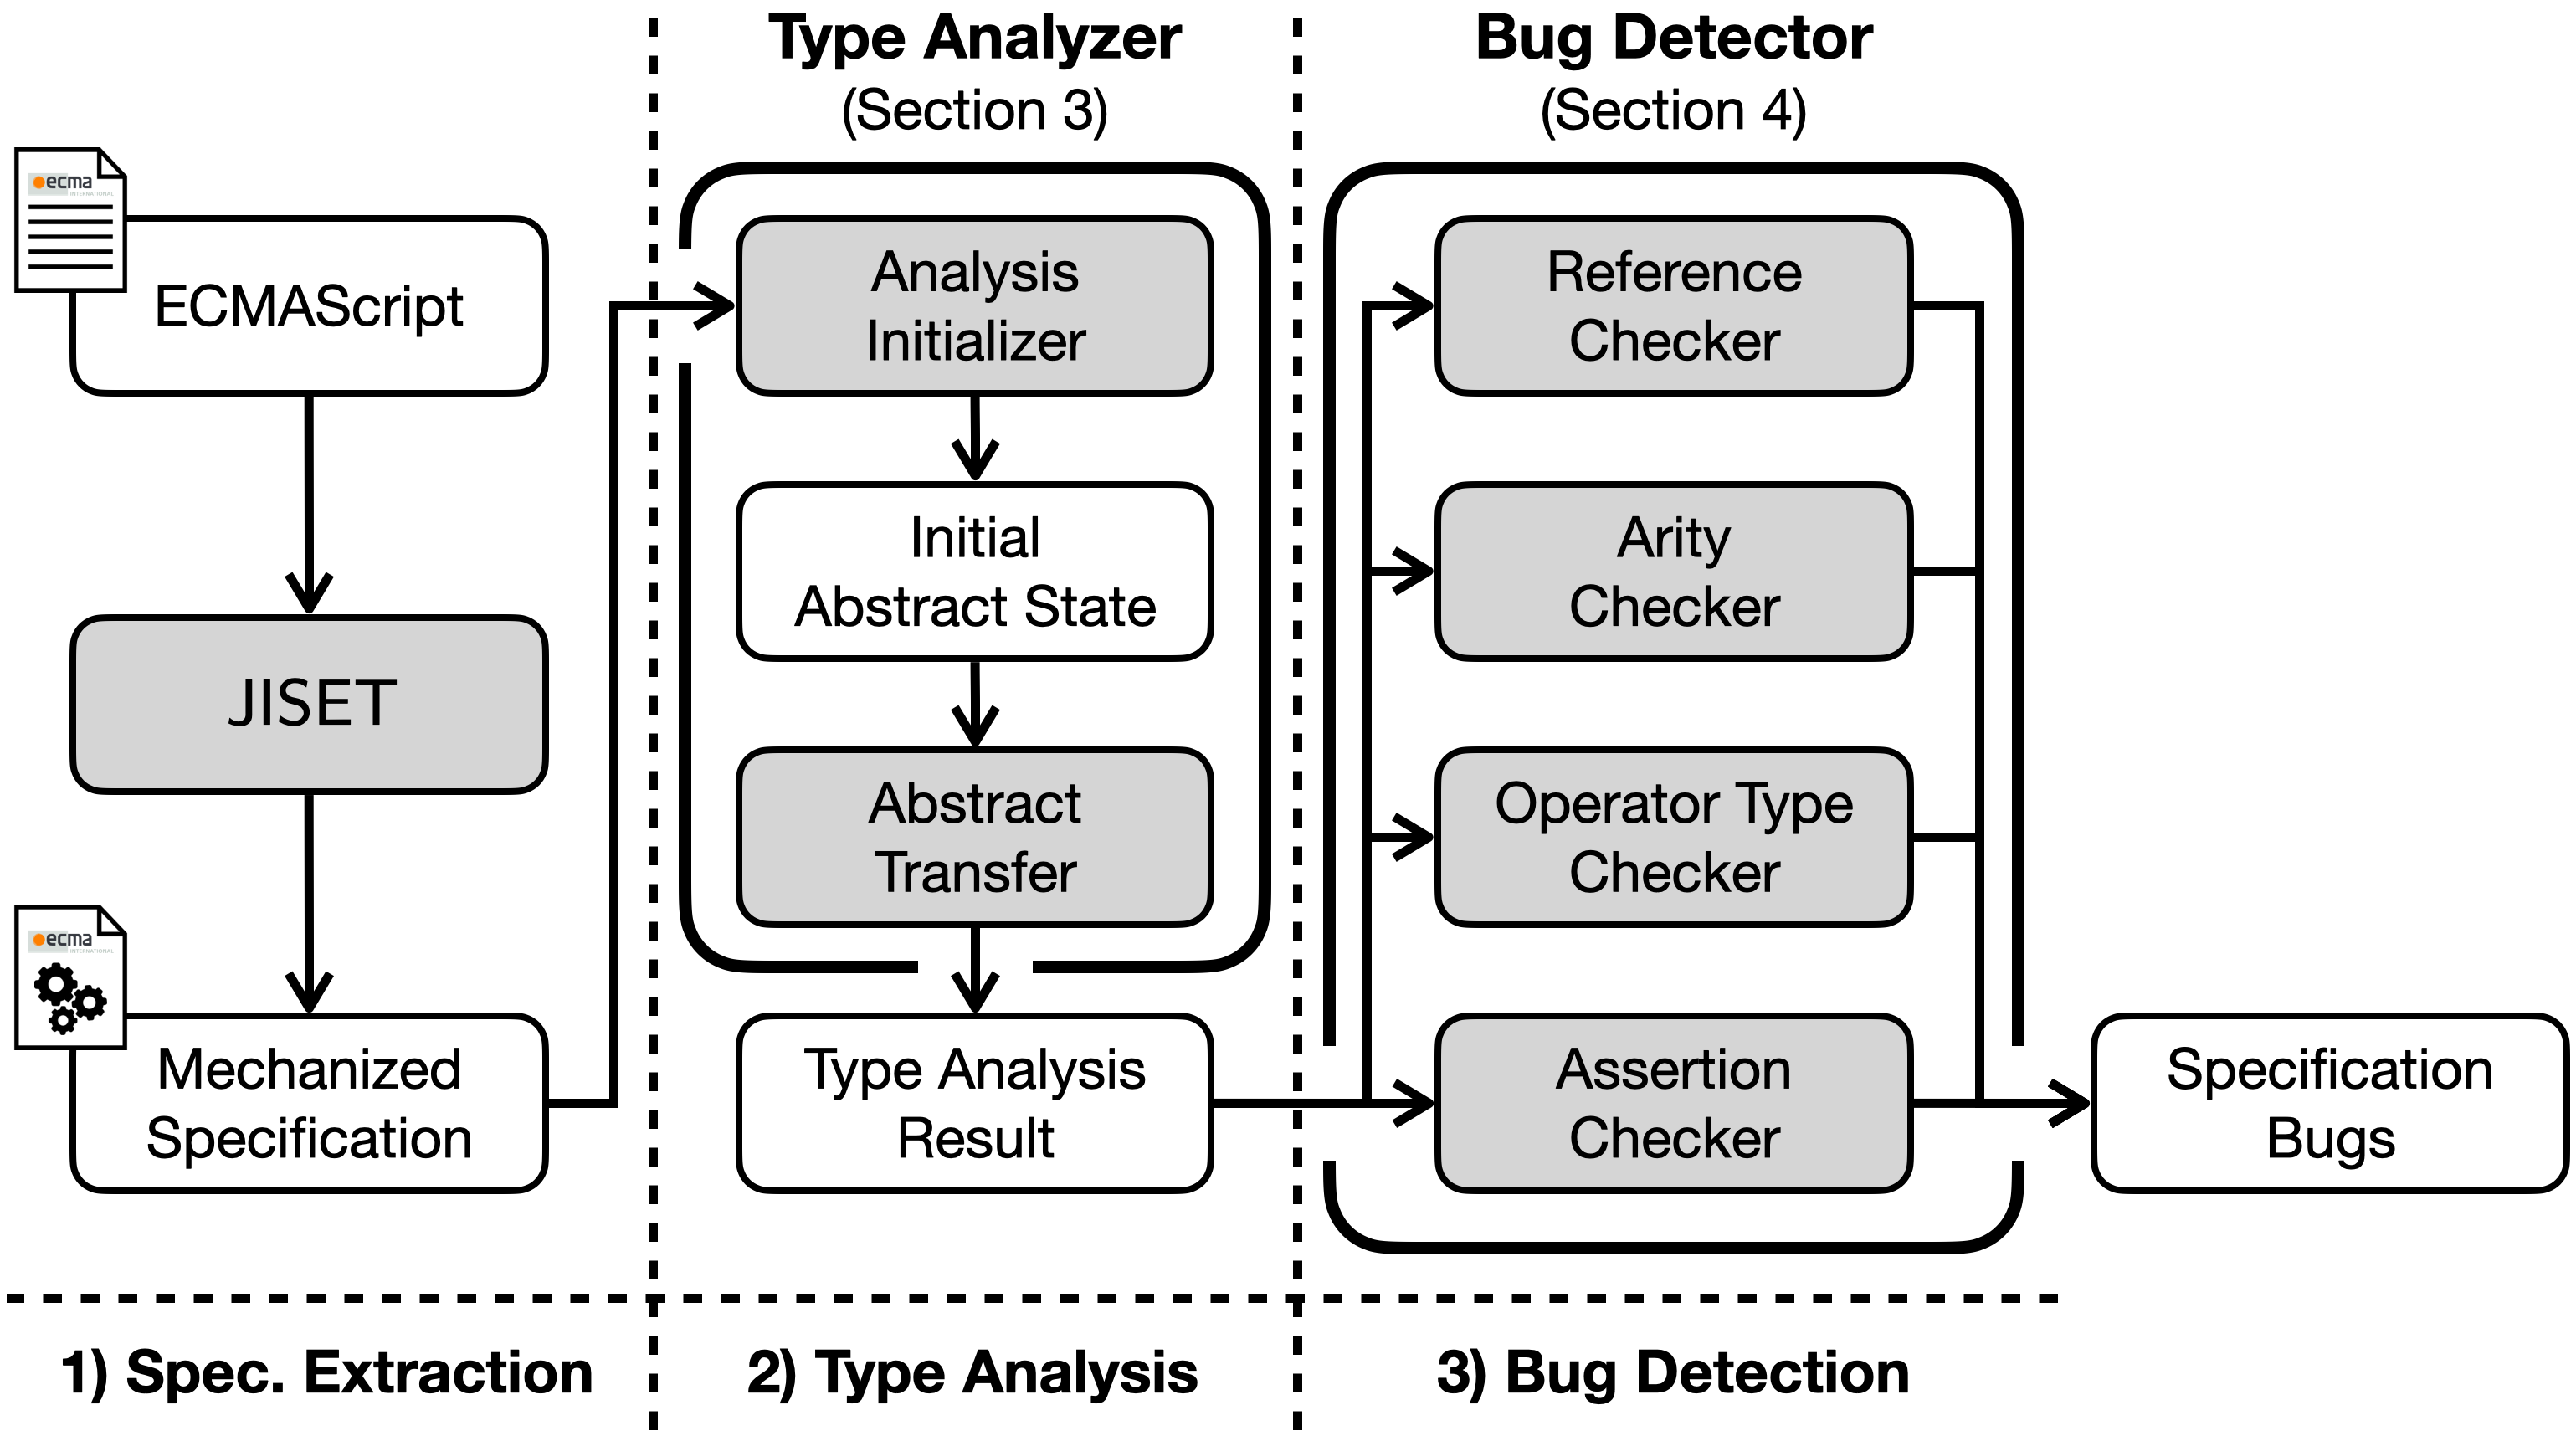
\includegraphics[width=\columnwidth]{img/overall}
  \caption{$\tool$: a type analyzer and a bug detector for
  mechanized specifications extracted from ECMAScript by $\jiset$}
  \label{fig:overall}
  \vspace*{-1.5em}
\end{figure}

\begin{figure*}[t]
  \centering
  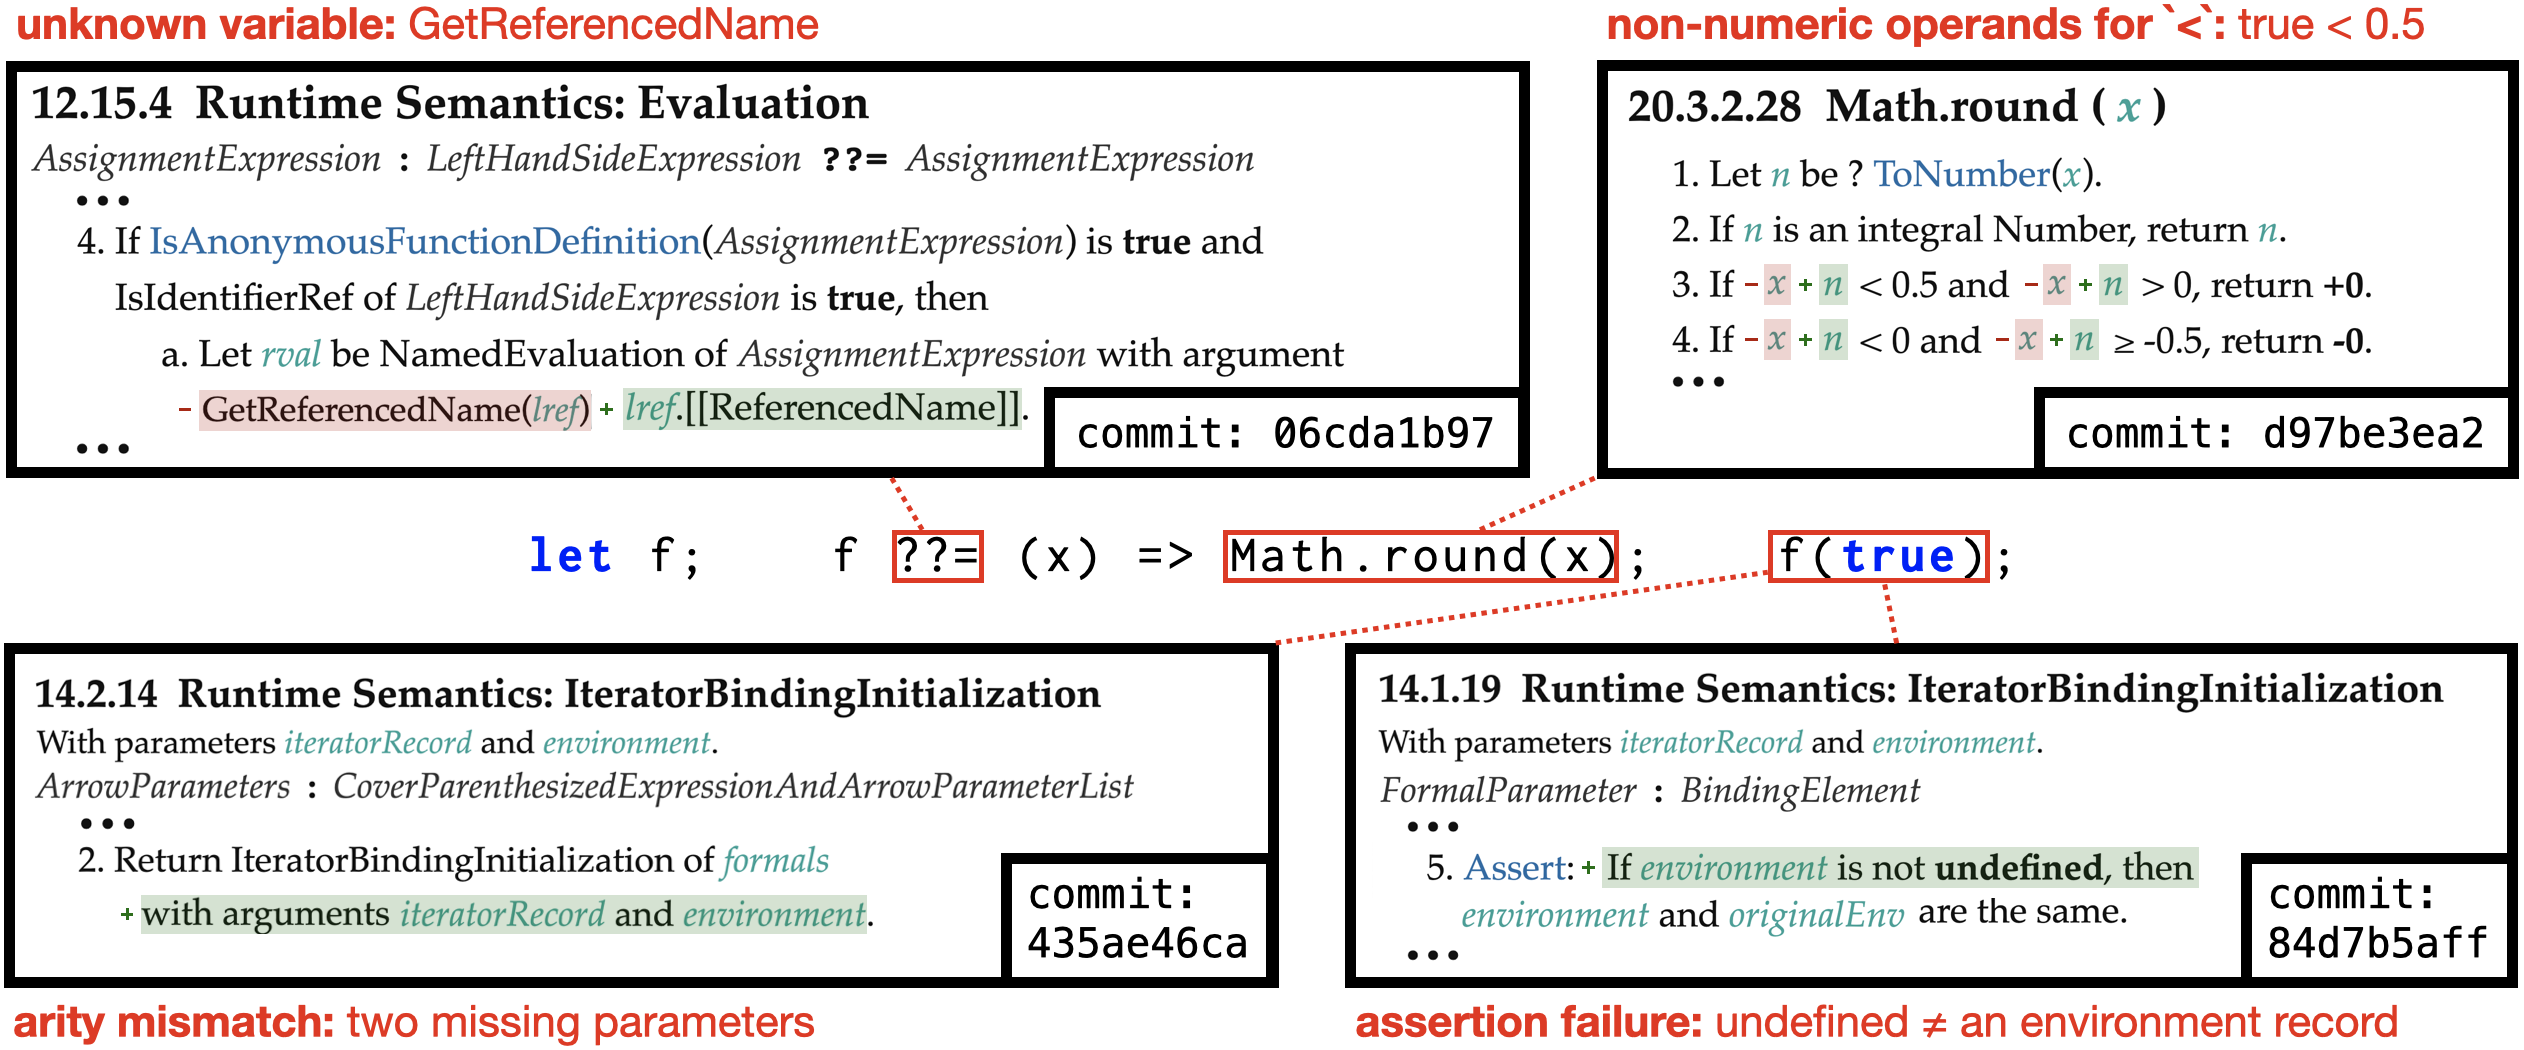
\includegraphics[width=.9\textwidth]{img/example}
%  \vspace*{-1.5em}
  \caption{An example JavaScript program with related previous specification
  bugs and their bug fixes}
  \label{fig:example}
  \vspace*{-1.5em}
\end{figure*}
% XXX
% \begin{lstlisting}[style=FigureJS]
% let f;    f ??= (x) => Math.round(x);    f(true);
% \end{lstlisting}

In this section, we demonstrate the overall structure of $\tool$ depicted in
Figure~\ref{fig:overall}.  It consists of three components:
1) specification extraction, 2) type analysis, and 3) bug detection.


\subsection{Specification Extraction}\label{sec:overview-spec-extract}
$\tool$ extracts the JavaScript syntax and semantics using $\jiset$
and extracts specification types from ECMAScript.

\paragraph{Syntax and Semantics}
ECMAScript describes the JavaScript syntax in an EBNF notation
and the semantics using abstract algorithms written in a structured natural language.
From ECMAScript, $\jiset$ synthesizes AST structures for syntax and 
compiles the abstract algorithms to $\ires$ functions with parameters
and local variables for semantics.  For example, the algorithm step
``\raisebox{-0.55ex}{
\includegraphics[width=0.55\columnwidth]{img/compile-example}}''
is compiled to an $\ires$ instruction $\kwlet \; \code{baseObj}\; \code{=}
\escaped\!  \code{ToObject(V.Base)}$.  To make it suitable for type analysis,
we modify $\ires$ as formally defined in Section~\ref{sec:ires}.

\paragraph{Types}
In addition to JavaScript types,
$\tool$ represents three kinds of specification types.
First, because ASTs are values in abstract algorithms, 
they can be stored in variables and passed as function arguments.
For ASTs, we use their production names as their
types and automatically link their corresponding syntax-directed algorithms to their fields.
Second, ECMAScript supports various record types and fields
whose possible values are defined in their corresponding tables.
For example, ``Table 9: Completion Record Fields'' in the latest
ECMAScript describes the fields of the completion records.
% The newest version contains tens of tables for record types, and they are backward compatible in general.
Thus, we manually model the fields of record types based on the tables
in the latest version and use them in a type analysis.
Third, for list-like structures, we define the empty list type
$\clist{}$ and parametric list types $\clist{\tau}$.

\subsection{Type Analysis}\label{sec:overview-type-analysis}

$\tool$ performs a type analysis with flow-sensitivity and
type-sensitivity for arguments.
Each function is split into multiple flow- and type-sensitive views, and an
abstract state stores mapping from views to corresponding abstract environments.
To handle views separately, we use a worklist algorithm.
The type analyzer consists of two sub-modules: an \textit{analysis initializer} and an
\textit{abstract transfer function}.

\paragraph{Analysis Initializer} It defines the initial abstract state and the
initial set of views for a worklist. ECMAScript provides three
kinds of abstract algorithms: \textit{normal}, \textit{syntax-directed}, and \textit{built-in}. 
As for entry points of type analysis, we use syntax-directed algorithms and built-in algorithms
because they have their parameter types.  For each entry point, the
initializer defines its abstract environment with parameter types and adds the
flow- and type-sensitive views of the entry point to the worklist.

\paragraph{Abstract Transfer Function} For each iteration, the abstract transfer function gets a
specific view from the worklist and updates the abstract environments of the next
views based on the abstract semantics.  It adds the next views to the worklist if
it changes their abstract environments, and the iteration finishes when
the worklist becomes empty.  To increase the analysis precision, we
perform a condition-based refinement for an abstract environment when the current
control point is a branch or an assertion as described in Section~\ref{sec:refine}.

\subsection{Bug Detection}\label{sec:overview-bug-detect}

To detect specification bugs utilizing the type analysis, we develop
four checkers in a bug detector.  We explain the targets of the checkers
with an example JavaScript program that contains related previous specification bugs and
their bug fixes, as shown in Figure~\ref{fig:example}.

\paragraph{Reference Checker} The example JavaScript program first defines a
variable \jscode{f} without initialization, which has the value \jscode{undefined}.
It then assigns an anonymous function to \jscode{f} using the operator \jscode{??=}.
While the corresponding \textbf{Evaluation} algorithm in Figure~\ref{fig:example}(a) originally
used the \textbf{GetReferencedName} algorithm to get a reference name on line 4.a,
a contributor removed the \textbf{GetReferencedName} algorithm and replaced all its
invocations with accesses of the field [[ReferencedName]] on October 28, 2020.
However, the contributor missed several cases including the semantics of
\jscode{??=}, which was fixed by another contributor on November 3, 2020.
Thus, the unknown variable bug for \textbf{GetReferencedName} lasted for 7 days,
which the reference checker can detect.

\paragraph{Arity Checker} The program finally calls \jscode{f} with an argument \jscode{true}.
During the initialization of the function call, \textbf{IteratorBindingInitialization}
in Figure~\ref{fig:example}(b) is executed with additional parameters \textit{iteratorRecord} and
\textit{environment} to assign argument values to parameters.
However, a contributor missed passing additional arguments to them on line 2 in
\textbf{IteratorBindingInitialization} of \textit{ArrowParameters} on September 6, 2018.
It caused an arity mismatch bug, which lasted for 533 days until another
contributor fixed it on February 20, 2020. The arity checker can detect such arity mismatches.

\paragraph{Assertion Checker} During the initialization of the function call,
\textbf{IteratorBindingInitialization} of \textit{FormalParameter} in Figure~\ref{fig:example}(c)
contains another bug.
Even though the additional \textit{environment} parameter may contain \jscode{undefined},
a contributor did not consider it on line 5 in the initial commit of the open development process
on September 22, 2015.  It caused an assertion failure bug, which lasted for 1,297 days until another
contributor fixed it on April 10, 2019.
The assertion checker can detect such assertion failures.


\paragraph{Operand Checker} After the function call initialization, the
parameter \jscode{x} has the value \jscode{true}, and \jscode{Math.round} in Figure~\ref{fig:example}(d) is invoked
with the argument \jscode{true}.  The \jscode{Math.round} built-in library first
converts the given parameter \textit{x} to its corresponding number value
\textit{n} using \textbf{ToNumber}, and performs the remaining
steps using \textit{n}.  However, a contributor mistakenly used
\textit{x} instead of \textit{n} on lines 3 and 4 on September 11, 2020.
This bug caused the algorithm to compare the boolean value \jscode{true} with the
numeric value 0.5 or 0 in the example code.
This bug lived for two days until another contributor fixed it, and
the operand checker can detect them.

In the remainder of this paper, we explain the details of how to perform type
analysis for $\ires$ functions and how to increase the analysis precision using
the condition-based refinement (Section~\ref{sec:analyzer}) and how to detect
type-related specification bugs (Section~\ref{sec:checker}).  After we evaluate $\tool$
(Section~\ref{sec:eval}), we discuss related work (Section~\ref{sec:related})
and conclude (Section~\ref{sec:conclusion}).

\section{Parser Generator}\label{sec:parser}

In this section, we introduce a way to automatically generate JavaScript parsers
from given ECMAScript specifications. First, we explain \( \bnfes \), an extension
of Backus-Naur form(BNF) used in ECMAScript to describe lexical and
syntactic grammars of JavaScript. We propose a recursive descent parser generator
that both supports backtracking and lookahead tokens to correctly support
\( \bnfes \) notations. We implement our idea by extending Scala parser combinators.
The implementation also supports the automatic semicolon insertion,
one of the most distinctive parsing features in ECMAScript.

\subsection{\( \bnfes \): Grammars for ECMAScripts}

Backus-Naur form(BNF) is proposed to represent context-free grammars(CFGs).
ECMAScript provides their lexical and syntactic grammars using \( \bnfes \),
an extension of BNF for ECMAScript.
It consists of a number of \textit{productions} with the following forms:
\[
  \NT{A}(\param_1, \cdots, \param_k) ::=
  (\cond_1 \Rightarrow)^? \rhs_1 \mid
  \cdots \mid
  (\cond_n \Rightarrow)^? \rhs_n
\]
The left-hand side represents a parametric non-terminal \( \NT{A} \) with
multiple boolean parameters \( \param_1, \cdots, \param_n \).
If a non-terminal takes no parameters, parenthesis are omitted for the brevity.
A production has multiple right-hand sides with optional conditions.
A condition \( \cond \) is either a boolean parameter \( \param \)
or its negation \( ! \param \).
For example, consider the following production:
\[
  \NT{A}(\param) ::= \param \Rightarrow \T{a}
  \mid \; !\param \Rightarrow \T{b}
  \mid  \T{c}
\]
Then, \( \NT{A}(\kwt) \) means \( \T{a} \mid \T{c} \)
and \( \NT{A}(\kwf) \) means \( \T{b} \mid \T{c} \).

Each right-hand side \( \rhs \) is a sequence of the following symbols:
\begin{itemize}
  \item \( \boxed{\epsilon} \): empty sequence
  \item \( \boxed{\T{a}} \): terminal symbols
  \item \( \boxed{\NT{A}(\argument_1, \cdots, \argument_k)} \): non-terminal symbols
  \item \( \boxed{\symb?} \): optional symbols
  \item \( \boxed{\pm \symb} \): positive/negative lookahead symbols
  \item \( \boxed{\symb \butnot \symb'} \): exclusive symbols
  \item \( \boxed{\nolt} \): no line-terminator symbols
\end{itemize}

The empty sequence \( \epsilon \) passes without any conditions
and a terminal symbol is any token.
A non-terminal symbol \( \NT{A}(\argument_1, \cdots, \argument_k) \)
takes multiple arguments and each of them \( \argument_i \) is
a boolean value \( \kwt \), \( \kwf \) or a parameter \( \param_i \).
An optional symbol \( \symb? \) is same with \( \symb \mid \epsilon \).
A positive(negative) lookahead symbol \( +\symb \)(\( -\symb \))
checks that the symbol \( \symb \) succeeds(fails) and
\textit{never consumes any input}.
The exclusive symbols \( \symb \butnot \symb' \)
first checks that the symbol \( \symb \) succeeds
and then checks that the parsing result does not correspond to \( \symb' \).
The no-line terminal symbol \( \nolt \) is a special symbol
that restricts the white spaces between two other symbols.

\begin{figure}
  \centering
  \[
    \begin{array}{l}
      \NT{ArrayLiteral}(Yield, Await) ::=\\
      \qquad \T{[} \; Elision? \; \T{]}\\
      \qquad \T{[} \; ElementList(Yield, Await) \; \T{]}\\
      \qquad \T{[} \; ElementList(Yield, Await) \; \T{,} Elision? \; \T{]}\\
    \end{array}
  \]
  \caption{ArrayLiteral production in \( \bnfes \).}
  \label{fig:array-literal-bnfes}
\end{figure}

For example, 

\subsection{Lookahead Parsers}

Our goal is to automatically generate JavaScript parsers from ECMAScript
grammars written in \( \bnfes \). There are several options for parser generators;
ANTLR, Lex/Yacc, Bison, and PEG. Among them, we decided to use
Scala parser combinators defined under \textit{parsing expression grammars(PEG)}.
PEG follows top-down (LL-style) parsing approaches and there are two different
categories; predictive parser and recursive descent with backtracking.
Predictive parsers are widely used in general and LL(k) parsers are typical
examples of predictive top-down parsers.
They choose a right-hand sides based on predicting the next tokens in deterministic
manners. In the other hand, PEG is a recursive descent parser with
\textit{backtracking}. It visits each right-hand side in order and backtrack
into the previous rules when parsing fails.
Thus, it is possible to use each production itself as a parser
in PEG. Moreover, There are several reasons why we extend Scala parser combinator
to deal with ECMAScript lexers and grammars written in \( \bnfes \):

\begin{itemize}
  \item \textbf{Context-Sensitive Tokens} ECMAScript tokens are context-sensitive
    because of the JavaScript regular expressions and template strings.
    For example, the code \( \code{/x/g} \) might be a single regular expression token
    or four tokens that represent division by variables \( \code{x} \) and \( \code{g} \)
    depending on enclosing contexts. Thus, lexers should be evaluated during the parser
    not before the parser. Scala parser combinators also treat lexers as parsers thus
    it is possible to use appropriate lexers depending on the parsing contexts.
  \item \textbf{\( \bnfes \) Symbols} PEG is suitable grammars to represent
    \( \bnfes \) symbols. We will explain detailed conversion from
    \( \bnfes \) grammars into Scala parser combinators in section~\ref{sec:convert-bnfes}.
  \item \textbf{Multiple Starting Non-terminals} After ECMAScript 6, grammars support
    both scripts and modules as starting point of parsers. In Scala parser combinators,
    it is possible to parse input string using any non-terminals as parsers.
  \item \textbf{Parsing in Run-time} JavaScript supports \( \code{eval} \)
    function that parses given JavaScript String values into codes and evaluates them.
    Moreover, there is special phrases ``the \( N \) that is \textit{covered by}
    \( P \)'' in syntax-directed abstract algorithms.
    It means that the syntax tree \( P \) is parsed with generalized parsers because
    it needs evaluation contexts to correctly choose specific parsers.
    When the interpreter meets the above phrase, the specific parsers are now
    decided into \( N \) thus we should parse again the given syntax tree \( P \) with
    the non-terminal \( N \) in run time.
\end{itemize}

\subsubsection{Prioritized choices}
However, unfortunately, there is fundamental problem in PEG-based parsers;
\textit{prioritized choices}.
In PEG, the pipe operator ( \( \mid \) ) denotes a prioritized choice,
unlike CFG that deals with it in non-deterministic manners.
It means that PEG always pick the first success right-hand side even though
there exist other success choices in remaining right-hand sides.
While ECMAScript grammars are deterministic languages, some non-terminals
accepts multiple right-hand sides for a given input strings.
It distort the meaning of ECMAScript grammars.
For example, consider the following simplified grammars for JavaScript expressions:
\[
  \begin{array}{r@{~}c@{~}l}
    \NT{A} &::=& \NT{T} \T{;} \mid \NT{A} \; \T{+} \; \NT{T} \T{;} \\
    \NT{T} &::=& \T{a} \mid \T{a} \T{(} \T{b} \T{)}\\
  \end{array}
\]
While it represents deterministic grammar, the non-terminal \( \NT{T} \)
should accept both right-hand sides if the given string is \( \code{a(b);} \).
However, PEG-based parser fails to parse it
because the first right-hand side \( \T{a} \) is always tried
first in the non-terminal \( \NT{T} \).
Thus, the latter one \( \T{a} \T{(} \T{b} \T{)} \) is not reachable in PEG.
A simple solution is to change the order of right-hand sides;
\( \NT{T} ::= \T{a} \T{(} \T{b} \T{)} \mid \T{a} \).
However, it is not easy to ensure which order is correct
because their inclusion relationship should be calculated.
Moreover, some productions are not possible to resolve them
by simply re-ordering right-hand sides:
\[
  \begin{array}{r@{~}c@{~}l}
    \NT{A} &::=& \NT{B} \; \T{b}\\
    \NT{B} &::=& \T{a} \mid \T{a} \; \T{b}\\
  \end{array}
\]
The non-terminal \( \NT{A} \) should successfully parse two strings \( \code{ab} \)
and \( \code{abb} \). However, the non-terminal \( \NT{A} \) accepts only
\( \code{ab} \) and it accepts only \( \code{abb} \) when \( \NT{B} \) has
reversed order. It means that we should re-structure
the above rules to accept both strings in traditional PEG grammars.

\subsubsection{Lookahead tokens}
To alleviate such problems, we propose \textit{lookahead parsers},
which is extended recursive descent parsers with backtracking and
\textit{lookahead tokens}.
It keeps track of the next possible tokens using statically
calculated first tokens of each symbols using algorithm in
Figure~\ref{fig:first-tokens}. For example, the following steps explain
how to utilize lookahead tokens during parsing processes with
the input \( \code{a(b);} \):

\begin{figure}
\centering
\[
  \begin{array}{l@{~}c@{~}l}
    \rhsfirst{\symb_1 \cdots \symb_n} &=& \symbfirst{\symb_1} \firstplus
    \symbfirst{\symb_2 \cdots \symb_n}\\
    && \text{where} \; x \firstplus y = \left\{
    \begin{array}{ll}
      x \cup y & \text{if} \; \emptyfirst \in x\\
      x & \text{otherwise}\\
    \end{array}
    \right.\\
    \symbfirst{\epsilon} &=& \{ \emptyfirst \}\\
    \symbfirst{\T{a}} &=& \{ \T{a} \} \\
    \symbfirst{\NT{A}(\argument_1, \cdots, \argument_k)} &=&
    \rhsfirst{\rhs_1} \cup \cdots \cup \rhsfirst{\rhs_n}\\
    && \text{where} \; \NT{A}(\argument_1, \cdots, \argument_k) =
    \rhs_1 \mid \cdots \mid \rhs_n\\
    \symbfirst{\symb?} &=& \symbfirst{\symb} \cup \{ \emptyfirst \}\\
    \symbfirst{+\symb} &=& \symbfirst{\symb}\\
    \symbfirst{-\symb} &=& \{ \emptyfirst \}\\
    \symbfirst{\symb \butnot \symb'} &=& \symbfirst{\symb}\\
    \symbfirst{\nolt} &=& \{ \emptyfirst \}\\
  \end{array}
\]
\caption{Over-approximated first tokens of \( \bnfes \) symbols}
\label{fig:first-tokens}
\end{figure}

\Tree[.\(\NT{A}[\emptyfirst]\)
[.\(\NT{T}\T{;}[\emptyfirst]\)
[.\(\NT{T}[\T{;}]\)
\sout{\(\T{a}[\T{;}]\)}
[.\(\T{a}\T{(}\T{b}\T{)}[\T{;}]\)
[.\(\T{a}[\T{(}]\) \(\boxed{\T{a}}\) ]
[.\(\T{(}\T{b}\T{)}[\T{;}]\)
[.\(\T{(}[\T{b}]\) \(\boxed{\T{(}}\) ]
[.\(\T{b}\T{)}[\T{;}]\)
[.\(\T{b}[\T{)}]\) \(\boxed{\T{b}}\) ]
[.\(\T{b}\T{)}[\T{;}]\)
[.\(\T{)}[\T{;}]\) \(\boxed{\T{)}}\) ] ] ] ] ] ]
[.\(\T{;}[\emptyfirst]\)
\(\boxed{\T{;}}\) ] ] ]

Each node \( \symb^*[\la] \) denotes a sequence of symbols \( \symb^* \) with
lookahead tokens \( \la \), which is the set of tokens.
The parsing process follows pre-order traversals.
It starts from the starting non-terminal \( \NT{A} \) with the special
lookahead \( \emptyfirst \), which denotes the end of inputs.
Then, it visits the first right-hand side \( \NT{T} \T{;} \) with the same lookahead.
Each symbol will be visited with the corresponding lookahead, that is the
first tokens of the right next symbol.
For example, for the symbol \( \NT{T} \), the next symbol is \( \T{;} \)
and its first token is itself. Thus, the parser visits \( \NT{T} \)
with the lookahead \( \T{;} \). The most important point in this parsing process
is the first right hand side \( \T{a} \) of the non-terminal \( \NT{T} \).
It is visited with the lookahead \( \T{;} \) but the next token of the input string
\( \code{a(b);} \) is \( \code{(} \) not \( \code{;} \).
Thus, it fails to parse the input string even though the current token is
same with the terminal \( \T{a} \).
Thus, the parser could visit the next right-hand side \( \T{a}\T{(}\T{b}\T{)} \)
and finally the input \( \code{a(b);} \) is successfully parsed.

We formally define semantics of lookahead parsers
in Figure~\ref{fig:laparser} by converting them into the given parsers.
The helper function \( \getlap{\la} \) generates a parser by combining all
tokens in the lookahead \( \la \) using prioritized choices.
In this case, the order does not change the semantics of lookahead parsers
because \( \getlap{\la} \) just check whether it contains the given token or not.

\begin{figure}
\centering
\[
  \begin{array}{l@{~}c@{~}l}
    (\symb_1 \cdots \symb_n)[\la] &=&
    \symb_1[\symbfirst{\symb_2 \cdots \symb_n} \firstplus \la] \;
    (\symb_1 \cdots \symb_n)[\la]\\
    \epsilon[\la] &=& +\getlap{\la}\\
    \T{a}[\la] &=& \T{a} \; +\getlap{\la} \\
    \NT{A}(\argument_1, \cdots, \argument_k)[\la] &=&
    \rhs_1[\la] \mid \cdots \mid \rhs_n[\la]\\
    && \text{where} \; \NT{A}(\argument_1, \cdots, \argument_k) =
    \rhs_1 \mid \cdots \mid \rhs_n\\

    \symb?[\la] &=& \symb[\la] \mid \epsilon[\la]\\
    (\pm\symb)[\la] &=& \pm(\symb[\la]) \\
    (\symb \butnot \symb')[\la] &=& \symb[\la] \butnot \symb'\\
    \nolt &=& \nolt \; +\getlap{\la}\\
  \end{array}
\]
\caption{Formal semantics of lookahead parsers}
\label{fig:laparser}
\end{figure}

\subsection{Implementation}

We implement lookahead parsers by extending Scala parser combinators.
We define \( \code{LAparser} \) trait to represent lookahead parser
and it has two members; first tokens and a function from lookahead tokens into parsers
described in Figure~\ref{fig:first-tokens} and Figure~\ref{fig:laparser}, respectively.
There exists two different issues in implementing the lookahead parsers in Scala
to treat ECMAScript syntax written in \( \bnfes \).

\paragraph{Performances} One of critical weak points of recursive descent parsing
with backtracking is its performance. Basically, it needs exponential time related
to the input size because of the backtracking mechanism. Fortunately,
Ford et al~\cite{packrat} proposed Packrat parsing that provides linear
time complexity based on memoization technique. The main idea is that it treats
each parser as a function from the current input position into the parsing result.
Thus, it just memoizes each parser based on input positions. It dramatically reduces
the redundant parsing trials. In a similar way, we treat each lookahead parser as
a function from a pair of lookahead tokens and input positions into parsing results.

\paragraph{Left Recursions} The other issue is that recursive descent parsers
does not support left recursions in grammars. If a grammar has left recursions,
the parser falls into an infinite loop. To resolve this problem,
Warth et al~\cite{packrat-lr} proposed a way to support not only direct left
recursions but also indirect ones in Packrat parsing.
The basic idea is extends the memoization technique to support grow the parsing
results. We believe that it is conceptually possible to support direct and indirect
left recursions by applying the Warth's approach.
\inred{However, fortunately, it is not necessary to handle indirect left
recursions in order to deal with ECMAScript syntax because the all
versions of ECMAScript only have direct left recursions.}
Thus, we decided to just remove direct left recursions by defining sub productions
and carefully build the abstract syntax trees.

\subsubsection{AST generations}
We first automatically generate abstract syntax tree(AST) as Scala case classes
from the given \( \bnfes \) grammar that represents a version of ECMAScript.
For lexical grammars, their structures are not used in ECMAScript semantics
thus we gives them String types. For parser grammars, we need to
automatically synthesize a Scala file that has classes of syntax trees.
For each production \(
  \NT{A}(\param_1, \cdots, \param_k) ::=
  (\cond_1 \Rightarrow)^? \rhs_1 \mid
  \cdots \mid
  (\cond_n \Rightarrow)^? \rhs_n
\), the AST generator defines the \( \code{A} \) trait and
multiple sub classes \( \code{Ai} \) of \( \code{A} \) for right-hand sides.
Each class \( \code{Ai} \) has non-terminals as member variables and
its type is the corresponding non-terminal type. Additionally, only optional
non-terminal symbol has \( \code{Option[\_]} \) types.
For instance, the \( ArrayLiteral \) production
in~Figure\ref{fig:array-literal} automatically translated into the following
Scala classes:
\begin{lstlisting}[style=myScalastyle]
trait ArrayLiteral extends AST
case class ArrayLiteral0(x1: Option[Elision])
case class ArrayLiteral1(x1: ElementList)
case class ArrayLiteral2(x1: ElementList, x3: Option[Elision])
\end{lstlisting}

\subsubsection{Parser generations}\label{sec:convert-bnfes}
The next step is to automatically extract parsers from the given \( \bnfes \) grammar.
The conversion from \( \bnfes \) symbols into Scala codes is defined as follows:
\[
  \begin{array}{c|c}
    \bnfes \; \text{symbols} & \text{Scala codes}\\\hline\hline
    \epsilon & \code{MATCH}\\\hline
    \T{a} & \code{"a"}\\\hline
    \NT{A}(\argument_1, \argument_n) & \code{A(a1, .. , an)}\\\hline
    \symb? & \code{opt(s)}\\\hline
    \symb \butnot \symb' & \code{s\textbackslash s'}\\\hline
    \nolt & \code{NoLineTerminator}\\\hline
  \end{array}
\]
The \( \code{MATCH} \) denotes the empty sequence of lookahead parsers.
Each String literals are implicitly converted into lookahead parsers
through Scala implicit conversions. The \( \code{opt(s)} \) function
is same with \( \code{s | MATCH} \). We also define \( \code{\textbackslash} \)
operator between parsers to support exclusive parsers.
Finally, we support the \( \code{NoLineTerminator} \) parser.
It is a little bit tricky because it should hook the white space parsers
and check whether it contains line terminators.
However, it is possible in our approach because
we also automatically generates lexers not only parsers of ECMAScript syntax.
For the final result, the automatically synthesized parser from the
production \( ArrayLiteral \) in Figure~\ref{fig:array-literal} is defined
as the parsers defined in Figure~\ref{fig:array-literal}.

Moreover, we support automatic semicolon insertion algorithms as well.
It is the most distinctive parsing features in ECMAScript to parse more programs.
We extend our parser implementation to keep track of the right-most position
that fails to be parsed in the given input. In ECMAScript, the token at that
position is defined as \textit{offending token} and automatic semicolon insertion
algorithms are defined with such tokens. The algorithm is quite easy when we
already have the position offending tokens, because there are only three simple
rules. Thus, we just manually support them by following the rule in ECMAScript 2019.
Moreover, the rule is rarely changed because the only one sub-rule is added
after ECMAScript 5.1 written in 2011.

\section{Algorithm Compiler}\label{sec:compiler}
\begin{figure}
  \centering
  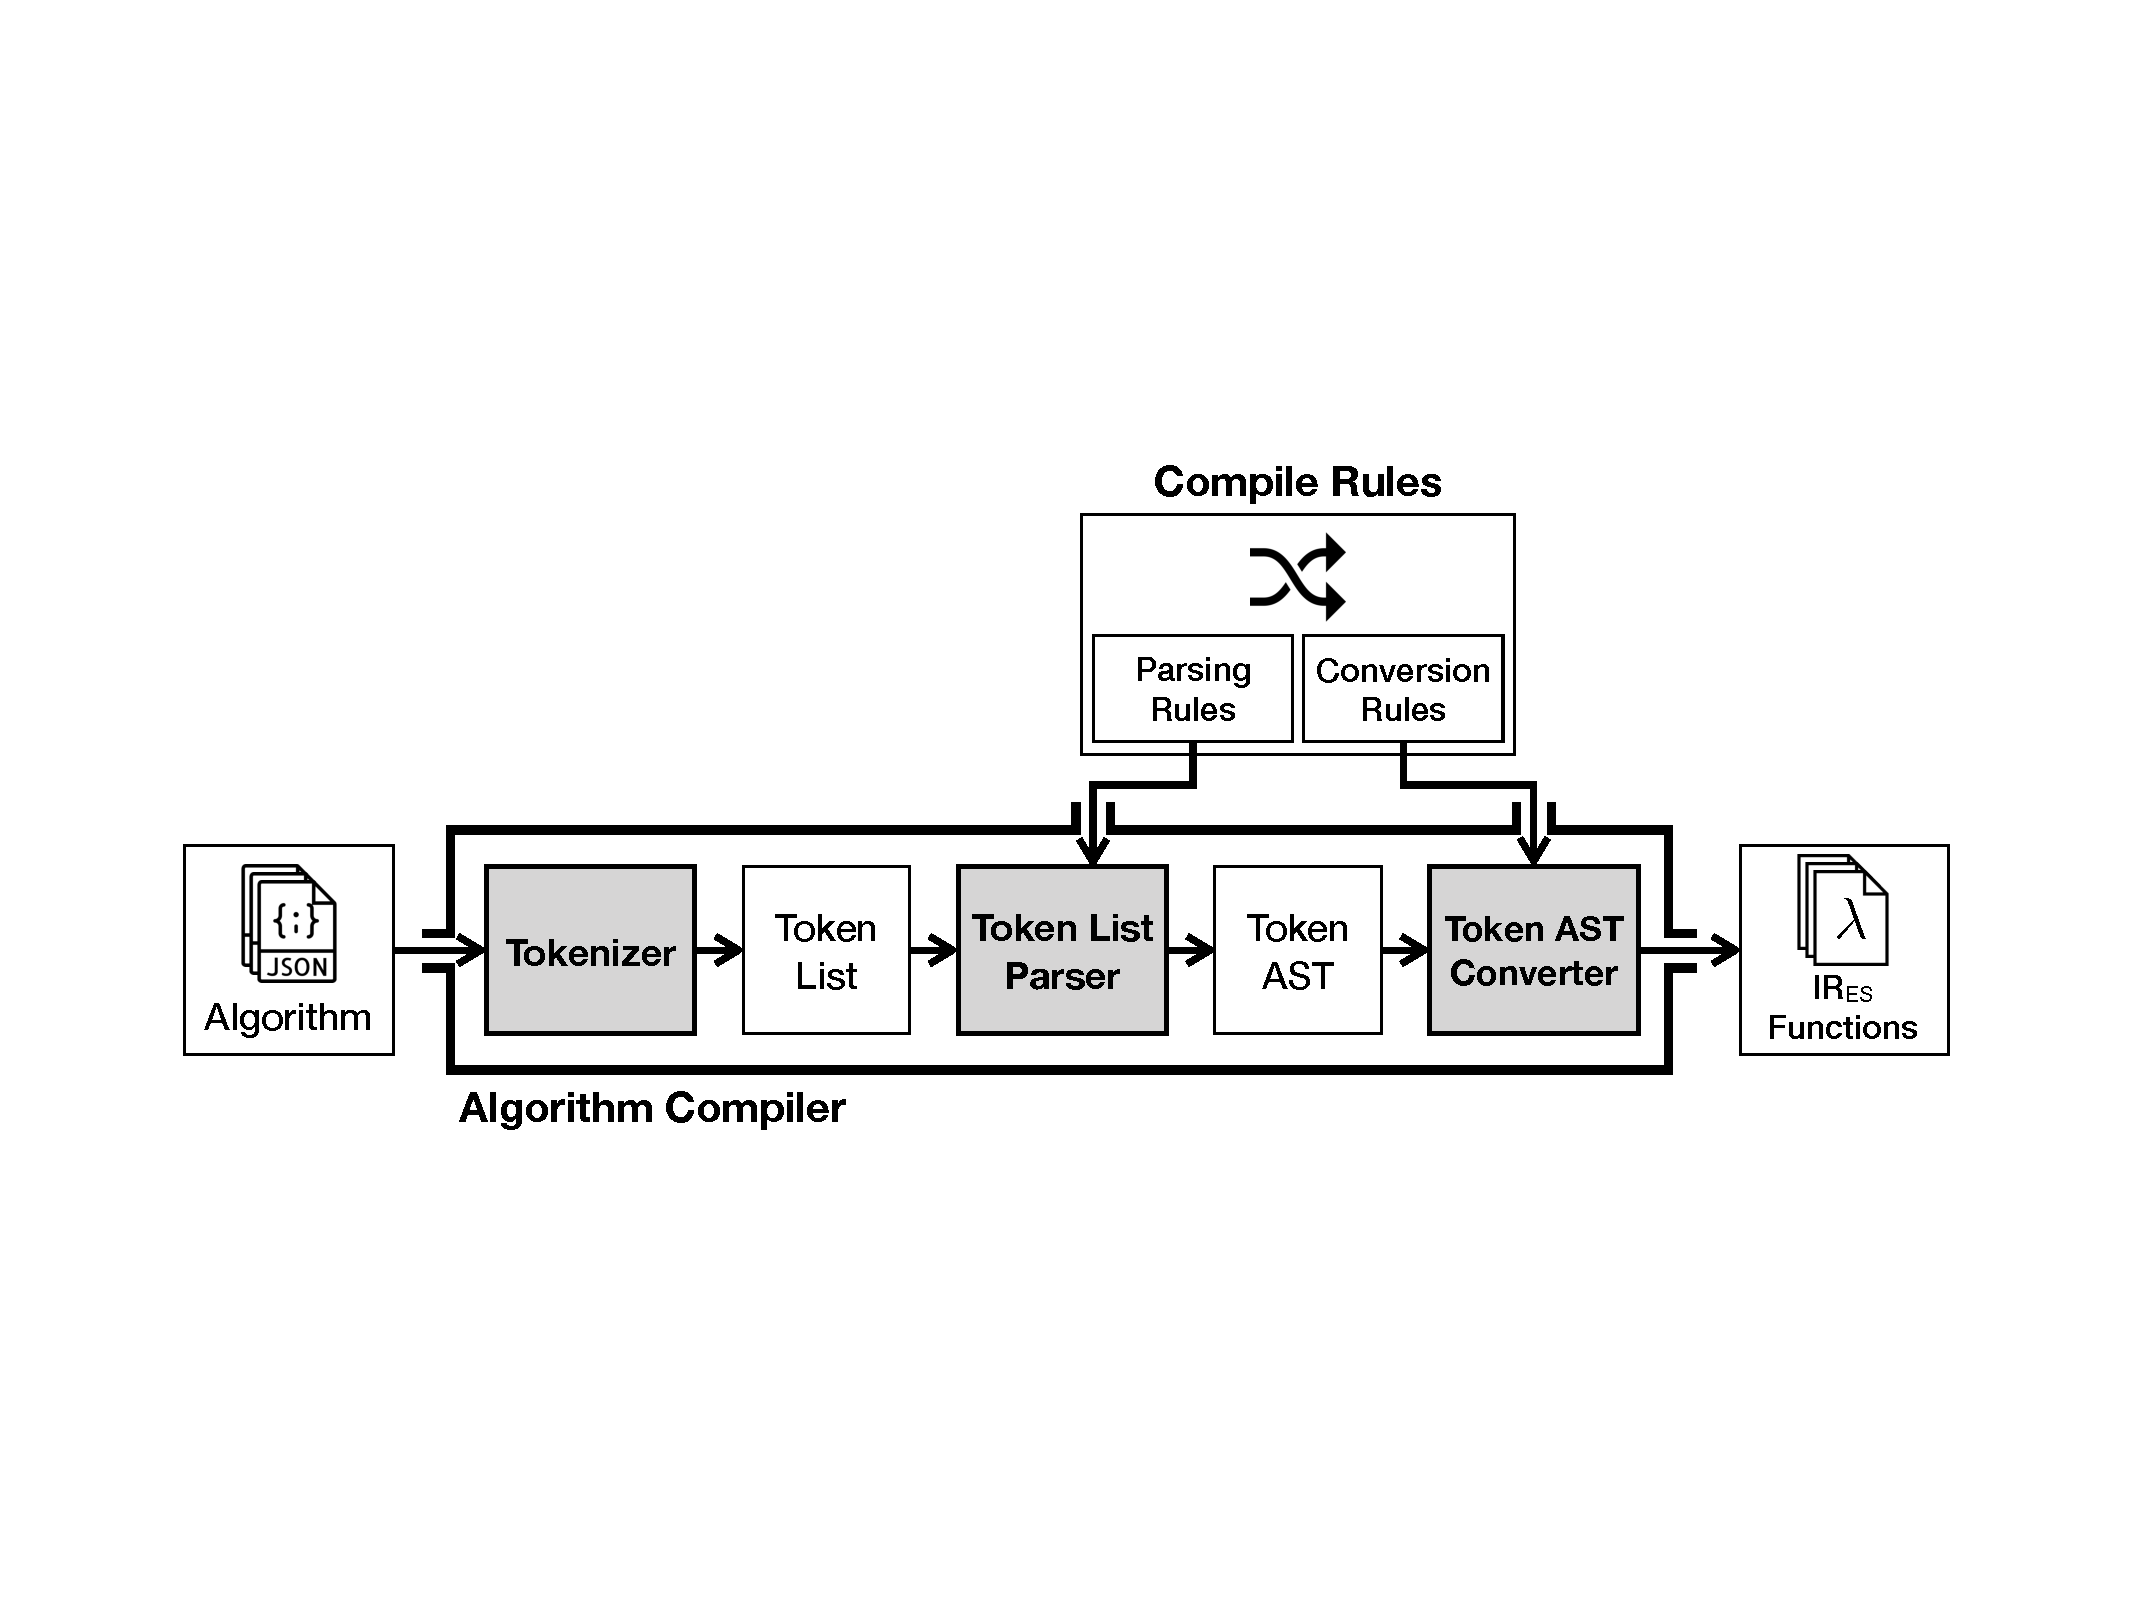
\includegraphics[width=0.48\textwidth]{img/algo-compiler.pdf}
  \caption{Overall structure of {\sf Algorithm Compiler}}
  \label{fig:algo-compiler}
\end{figure}

In this section, we explain {\sf Algorithm Compiler} that compiles
abstract algorithms to \( \ires \) functions as illustrated in
Figure~\ref{fig:algo-compiler}.

\subsection{Tokenizer}
Before compiling abstract algorithms, {\sf Tokenizer} first tokenizes each
abstract algorithm into a list of tagged tokens.  An algorithm consists of
ordered steps, and a step may contain sub-steps as well.  For example, the
\textbf{\small Evaluation} abstract algorithm in
Figure~\ref{fig:array-literal-eval}(a) has seven steps.  Moreover, the tokens of
each step have their own HTML tags and each tag has a meaning.  We keep such
HTML tag information for each token to construct more precise {\sf Compile
Rules}. If an HTML element is just a text without any explicit tags, it is
divided into multiple tokens and each token becomes a sequence of alphanumeric
characters or a single non-alphanumeric character.  For example, in the
\textbf{\small Evaluation} algorithm, \( \textbf{\code{"length"}} \) is a single
token with the HTML tag \( \code{<code>} \) and \( \code{Perform Set(} \) is
divided into three text tokens \( \code{Perform} \), \( \code{Set} \), and \(
\code{(} \).

Moreover, {\sf Tokenizer} flattens a structured step to a single token
list to handle multi-step statements easily.  Some statements in
abstract algorithms consist of multiple steps.  For example, the
\( \code{if}\!-\!\code{then}\!-\!\code{else} \) statement often consists of
two steps: one for the \( \code{then} \)-branch and the other
for the \( \code{else} \)-branch.  To treat them as a linear structure,
we introduce three special tokens to break down structured algorithms:
\( \tend \) denotes the end of a single step, and \( \tin \) and
\( \tout \) denote the start and the end of nested steps, respectively.
For example, the following left abstract algorithm is tokenized to the right
token list.
\[
  \begin{array}{lcl}
    \code{1. A}\\
    \code{2. B} &\Longrightarrow& \code{A} \tend \code{B} \tin \code{C} \tend \tout \tend\\
    \code{\ \ a. C}\\
  \end{array}
\]

After tokenizing abstract algorithms, {\sf Algorithm Compiler}
compiles token lists into \( \ires \) functions using
{\sf Token List Parser} and {\sf Token AST Converter}.
They depend on {\sf Compile Rules} and each compile rule
consists of a \textit{parsing rule} and a \textit{conversion rule}:
\begin{lstlisting}[style=myScalastyle]
val CompileRule = ParsingRule ^^ ConversionRule
\end{lstlisting}
For each compile rule, its parsing rule describes how to parse a given
token list into a structured token AST, and its conversion rule describes
how to convert the given token AST structure into an \( \ires \) component.
Now, we explain the token list parser and token AST converter with
parsing rules and conversion rules, respectively.


\subsection{Token List Parser}
The token list parser is defined with \textit{parsing rules}. A parsing rule
is a basic parsing rule or a composition of multiple parsing rules. The composition
\code{A | B} of two parsing rules \code{A} and \code{B} parses an input using
both rules and collects the longest matched results.  If both rules fail or
match the same length of the input, the composition fails.

We provide two kinds of basic parsing rules: \textit{tag-based rules} and
\textit{content-based rules}.  A tag-based rule just checks whether the next
token has a given tag.  For example, the tag-based parser \( \code{varT} \) and
\( \code{codeT} \) check whether the next token has the tag \( \code{<var>} \)
and \( \code{<code>} \), respectively.  A content-based parser checks whether
the next token is a text token and its content passes a given condition.  For
example, the string literal \( \code{"Perform"} \) denotes a content-based
parser that checks whether the next token is a text token with the content \(
\code{Perform} \).  We also define two content-based parsers \( \code{word} \)
and \( \code{number} \) that check whether the content of the next token
consists of only alphabets or numbers, respectively.  In addition, we provide
several helper functions such as the optional rule \code{A?} and
the positive(negative) predicate \code{+A}(\code{-A}).  For instance, the helper
function \( \code{repsep(A, B)} \) generates a new parsing rule that denotes
zero or more repetition of the parsing rule \( \code{A} \) using another parsing
rule \( \code{B} \) as a separator.

Consider the following example parsing rule for the step 5 of the
\textbf{Evaluation} algorithm in Figure~\ref{fig:array-literal-eval}(a).
\begin{lstlisting}[style=myScalastyle]
// statements
val Stmt = "Perform" ~ Expr ~ "." ^^ ...
// expressions
val Expr =
  // codes        // false literal
  codeT    ^^ ... |  "false"           ^^ ... |
  // variables       // additions
  varT     ^^ ... |  Expr ~ "+" ~ Expr ^^ ... |
  // function calls
  word ~ "(" ~ repsep(Expr, ",") ~ ")" ^^ ...
\end{lstlisting}
We omit the conversion rule for each compile rule for brevity.  The \(
\code{Stmt} \) compile rule  describes how to compile statements with a single
parsing rule, and the \( \code{Expr} \) compile rule describes how to compile
expressions with five parsing rules.  A token parser with the above rules parses
the step 5 of \textbf{Evaluation} to the following token AST:
\begin{center}
  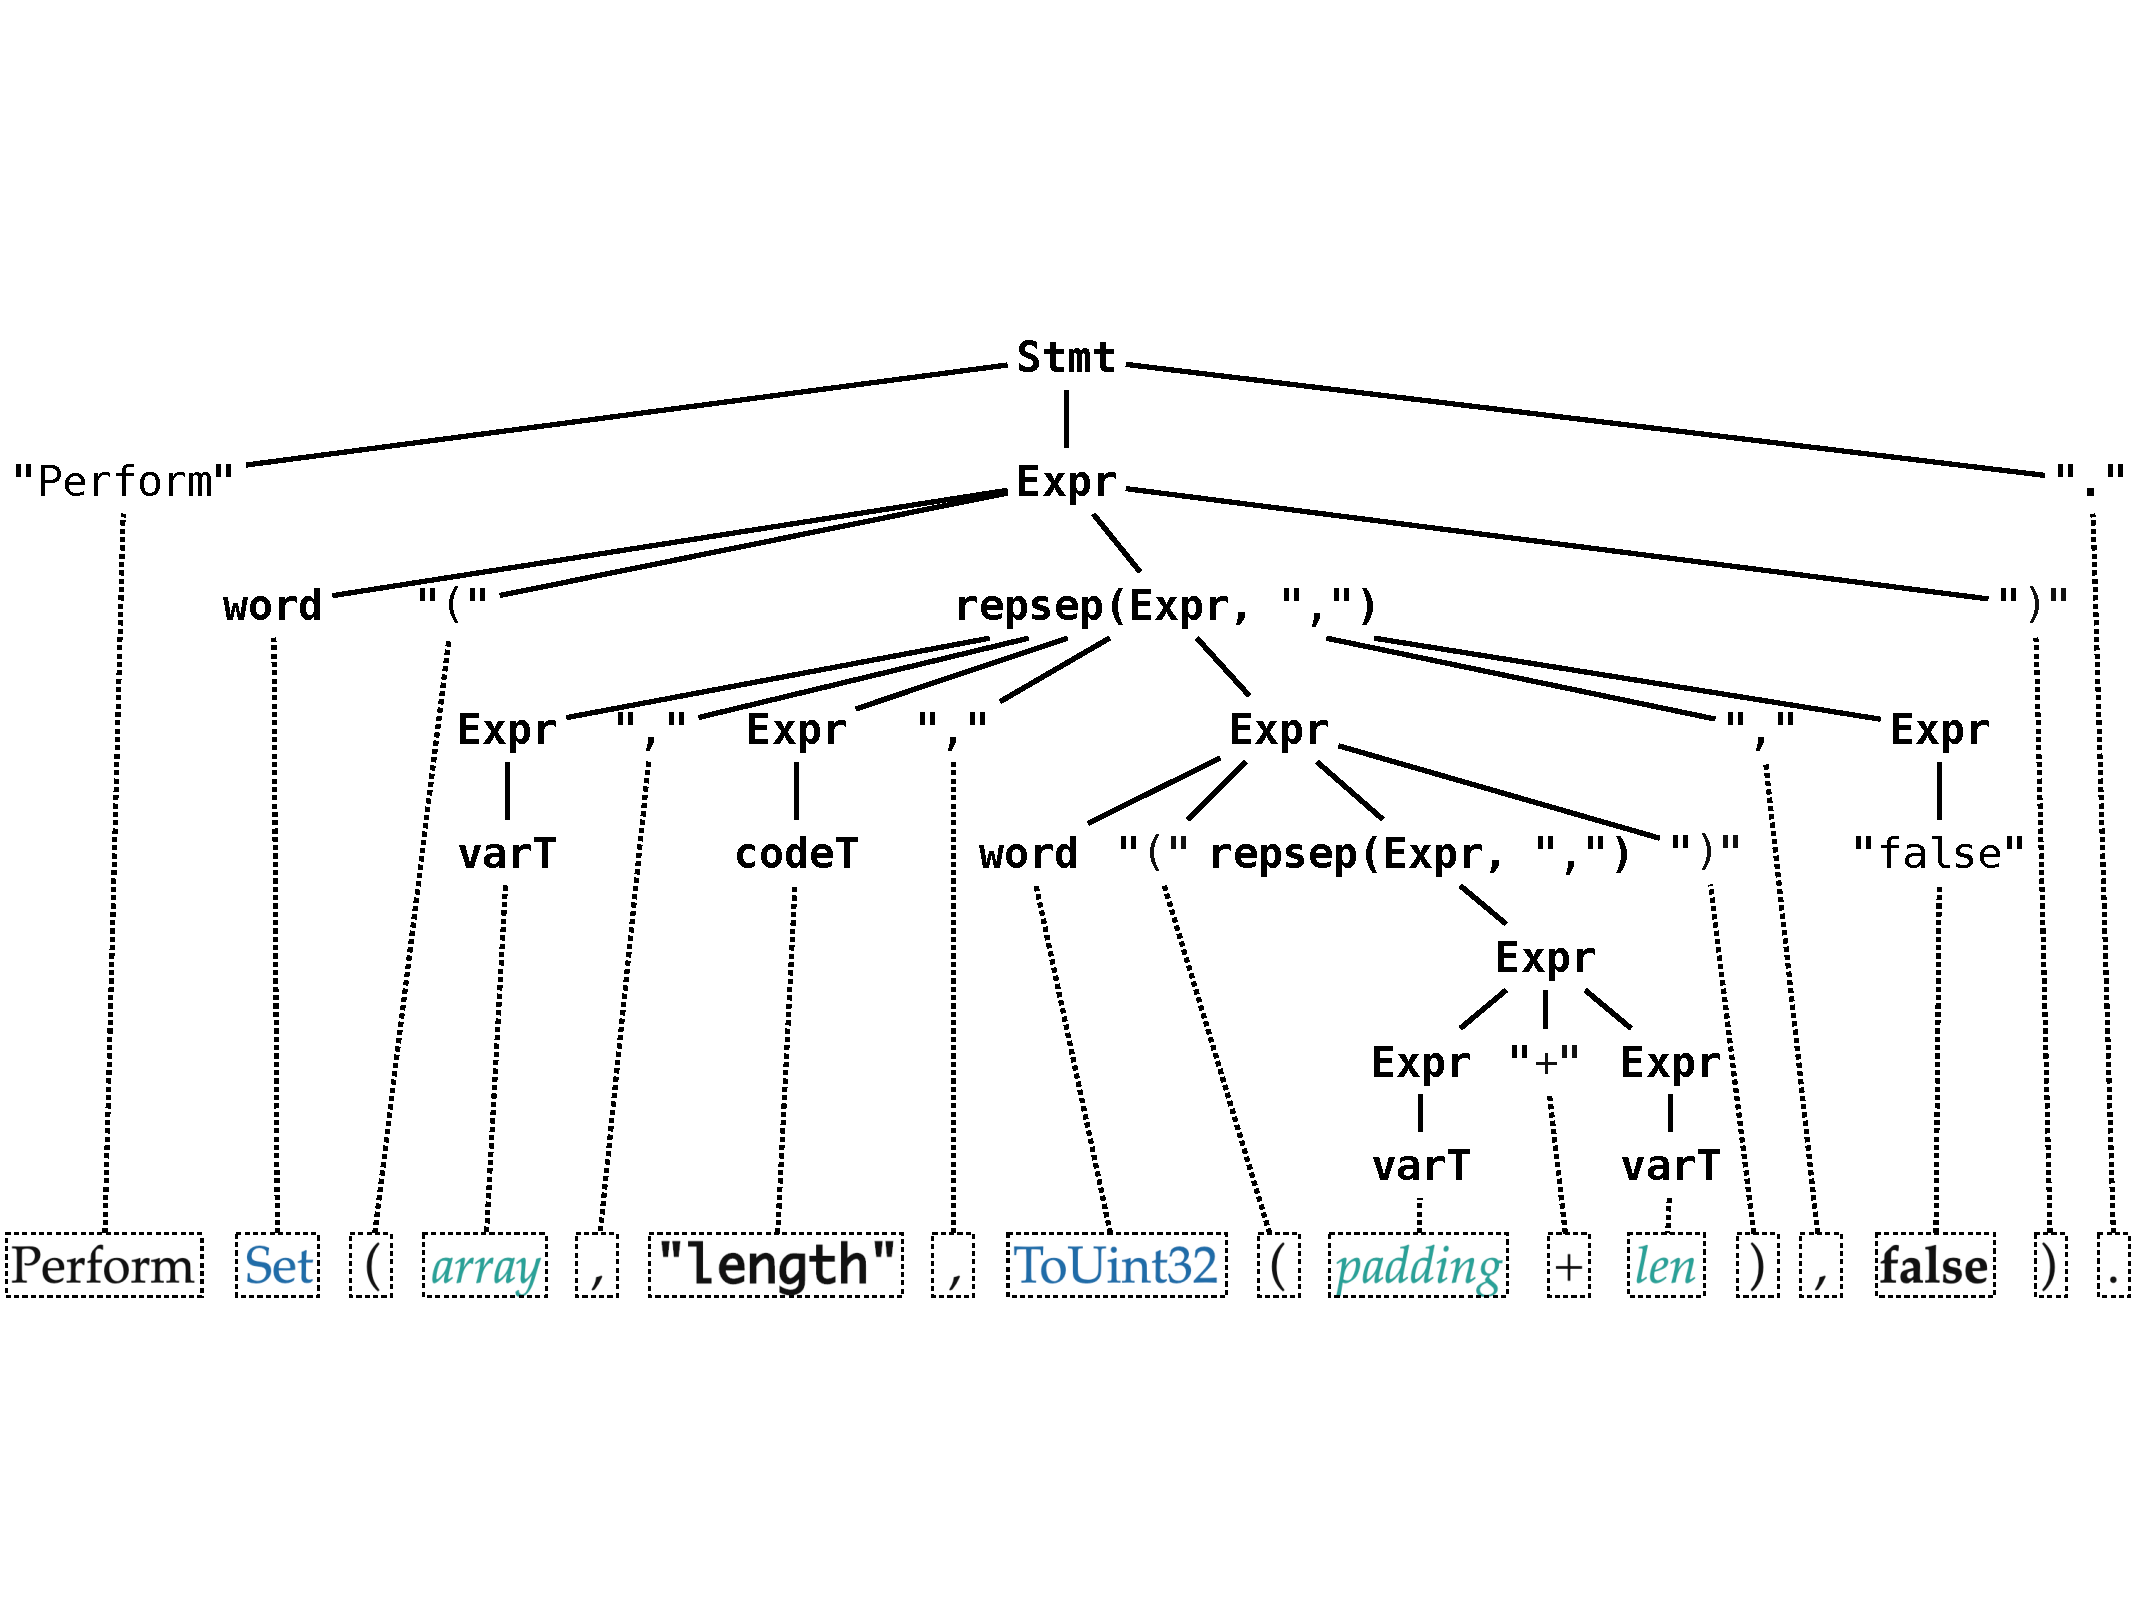
\includegraphics[width=0.5\textwidth]{img/token-ast.pdf}
\end{center}


\subsection{Token AST Converter}
\textit{Conversion rules} describe how to generate an \( \ires \) function for a
given token AST.  Each conversion rule is defined with its corresponding parsing
rule.  For basic parsing rules, their conversion rules always return the string
values of the contents in parsed tokens.  For example, the following conversion
rules are the omitted parts in the previous example for the step 5 of
\textbf{Evaluation}:
\begin{lstlisting}[style=myScalastyle]
// statements
val Stmt = ... ^^ { case _ ~ e ~ _ => IExpr(e) }
// expressions
val Expr =
  // codes      // false literal
  ... ^^ EStr | ... ^^ { _ => EBool(false) }            |
  // variables  // additions
  ... ^^ EId  | ... ^^ { case x ~ _ ~ y => EAdd(x, y) } |
  // function calls
  ... ^^ { case x ~ _ ~ y ~ _ => ECall(x, y) }
)
\end{lstlisting}
The conversion rule of the \code{Stmt} compile rule uses only the second sub
tree and constructs an \code{IExpr} \( \ires \) instruction.  For the second
sub-tree, the conversion rule of the fifth \code{Expr} compile rule is
applied. It constructs \code{ECall} \( \ires \) expression with the string value
of the first sub-tree and the sequence of the expressions of the third sub-tree.
In this way, the step 5 of \textbf{Evaluation} is converted to the following \(
\ires \) instruction whose beautified form is the seventh line
in Figure~\ref{fig:array-literal-eval}(b).
\begin{lstlisting}[style=ires]
IExpr(ECall(EId("Set"), List(
  EId(array), EStr("length"), ECall(EId(ToUint32), List(
    EAdd(EId("padding"), EId("len")))), EBool(false))))
\end{lstlisting}

We define \( \ires \) to represent abstract algorithms as its
functions with the following design choices:
\begin{itemize}[leftmargin=0.5cm]
\item \textbf{Dynamic typing:} Because each variable in abstract
algorithms is not statically typed, variables do not have their own
static types while each value of \( \ires \) has its dynamic type.

\item \textbf{Imperative style:} \( \ires \) represents algorithm steps
as imperative instructions in the sense that each instruction changes
the current state consisting of an environment and a heap.

\item \textbf{Higher-order functions with restricted scopes:}
In each function of \( \ires \), only global variables, parameters,
and its local variables are available, which means that a function
closure does not capture its current environment.  We use such
restricted scopes because they are enough to represent abstract
algorithms.

\item \textbf{Primitive values:} \( \ires \) supports ECMAScript primitive
values except ``symbols'' because symbols can be represented as singleton
objects.  Also, \( \ires \) provides the unique \( \code{absent} \) value to
represent the absence of parameters.  For example, when the optional second
parameter \textit{Elision} of \textbf{Evaluation} in
Figure~\ref{fig:array-literal-eval}(a) is absent, the parameter has the \(
\code{absent} \) value.

\item \textbf{Abstract data types:} \( \ires \) supports only three abstract
data types: \( \code{Record} \) for mappings from values to values,
\( \code{List} \) for sequential data, and \( \code{Symbol} \) for singleton
data.  For example, ECMAScript environment records are represented as \(
\code{Record} \) from string values to addresses that represent the
bindings of the string values.
\end{itemize}
We define the syntax of \( \ires \) that has 15 kinds of instructions and 26 kinds
of expressions with the notation \( \irinst \) and \( \irexpr \), respectively.
We also formally define its operational semantics \(
\irstate \vdash \irinst \Rightarrow \irstate \) for instructions and
\( \irstate \vdash \irexpr \Rightarrow (\irvalue, \irstate) \) for expressions,
where \( \irstate \) denotes a state and \( \irvalue \) denotes a value.
For presentation brevity, we omit the formalization of \( \ires \) in this paper
and include it in a companion report\inred{\cite{report}}.


\subsection{Implementation}
We implemented {\sf Algorithm Compiler} by extending the Packrat
parsing~\cite{packrat} library in Scala parser combinators. We modified the
meaning of the composition operator ( \( | \) ) to collect all the
longest matched results.  If a parser detects a step that cannot be parsed or
is parsed in multiple ways, it reports the step with parsing results.


\paragraph{Compile Rules}
\textsf{Algorithm Compiler} requires compile rules to compile given abstract
algorithms to \( \ires \) functions.  As already explained in
Section~\ref{sec:overview}, we found common patterns in the writing style of
abstract algorithms.  We manually defined general compile rules to represent
such a writing style with six different kinds as summarized in
Table~\ref{table:rules}.  The compile rule for statements, \( \code{Stmt} \),
generates \( \ires \) instructions.  The \( \code{Expr} \), \( \code{Cond} \),
and \( \code{Value} \) compile rules generate \( \ires \) expressions, but they
represent different contexts in ECMAScript; \( \code{Expr} \) represents a
context where any expression can appear, \( \code{Cond} \) denotes a context
where any boolean-valued expression can appear, and \( \code{Value} \)
represents a context where a fully evaluated value can appear.  The \( \code{Ty}
\) compile rule denotes type names and generates string primitives used in
object constructions.  The \( \code{Ref} \) compile rule represents references such as
identifier lookup and member accesses of objects, and it generates \( \ires \)
references.

\begin{table}[t]
  \centering
  \caption{General compile rules for ECMAScript}
  \label{table:rules}
\vspace*{-1em}
  \[
  \begin{array}{c?r|r|r|r|r|r}%|r}
      \text{Name}
      & \multicolumn{1}{c|}{\code{Stmt}}
      & \multicolumn{1}{c|}{\code{Expr}}
      & \multicolumn{1}{c|}{\code{Cond}}
      & \multicolumn{1}{c|}{\code{Value}}
      & \multicolumn{1}{c|}{\code{Ty}}
      & \multicolumn{1}{c}{\code{Ref}}\\\hline
      \text{\# Rules}
      & \inred{17}
      & \inred{16}
      & \inred{8}
      & \inred{11}
      & \inred{33}
      & \inred{7}
    \end{array}
  \]
\vspace*{-2em}
\end{table}


\paragraph{Global Setting}
{\sf AST-\( \ires \) Translator} uses global settings consisting
of \textit{ECMAScript data types} and \textit{built-in objects}.
Unlike compile rules, global settings depend on
ECMAScript versions. In this paper, we construct global settings only for the
latest ECMAScript, ES10.

ECMAScript describes data types with some fields and methods.
While the methods are like abstract algorithms, their semantics are
slightly different from abstract algorithms. They implicitly get their receiver objects as
arguments at callsites.  To mimic such an implicit behavior, we added a special
variable \( \code{this} \) as the first parameter of each method, and passed a
receiver object at its callsite by modifying \textsf{Algorithm Compiler}.  For
example, an Environment Record type has the \textbf{DeleteBinding (N)} method.
Thus, its corresponding \( \ires \) function has two parameters, the special
parameter \( \code{this} \) and a normal parameter \( \code{N} \), and the method call
\raisebox{-0.65ex}{
\includegraphics[width=0.17\textwidth]{img/method-call.png}}
in an abstract algorithm is compiled to the \( \ires \) instruction:
\code{(DclRec.DeleteBinding DclRec N)}.

In ECMAScript, built-in objects are pre-defined functions with several
built-in functions.  For example, \( \code{Array} \)
is the constructor of array objects, and its prototype
\( \code{Array.prototype} \) has built-in functions for array objects.
For instance, \( \code{[1,2,3].flat()} \) calls the
\( \code{Array.prototype.flat} \) built-in function with the array
\( \code{[1,2,3]} \).  Because built-in functions are also abstract
algorithms, each of them is automatically converted to an \( \ires \)
function.  However, the structures of built-in objects should be
manually implemented.  Thus, we implemented built-in objects in Scala
and connected their properties with the extracted \( \ires \) functions.
%
Some built-in objects that are explicitly referenced in abstract
algorithms are intrinsic objects, which have their own
aliased names summarized in Table~7 of Section~6.1.7.4
\textsf{Well-Known Intrinsic Objects}.  We extracted the alias
into \textsf{Global Setting} to utilize it during evaluation.

\section{Implementation}\label{sec:impl}

\todo

\section{Evaluation}\label{sec:eval}

We developed \( \tool \) as an open source tool\footnote{The URL of the tool is
anonymized due to a double-blind review process.}, and evaluated the tool
based on the following three research questions:
\begin{itemize}[leftmargin=0.5cm]
\item RQ1. \textbf{Coverage:} How much parts \( \tool \) automatically extract
the syntax and semantics from ES7 to ES10?
\item RQ2. \textbf{Check with Tests:} The syntax and semantics of the latest
version on ECMAScript (ES10) is compatible with official tests?
\item RQ3. \textbf{Forward Compatibility:} Is \( \tool \) applicable to language
features ready for inclusion in the next ECMAScript (ES11)?
\end{itemize}


\subsection{Coverage}

\begin{table}[t]
  \caption{Number of productions in specifications,
from \textit{all} of which \( \tool \) automatically generated parsers}
  \label{fig:syntax-all-version}
\vspace*{-1em}
\small
  \[
    \begin{array}{c?r|r|r|r?r}
      \textbf{Version}
      & \multicolumn{1}{c|}{\textbf{ES7}}
      & \multicolumn{1}{c|}{\textbf{ES8}}
      & \multicolumn{1}{c|}{\textbf{ES9}}
      & \multicolumn{1}{c?}{\textbf{ES10}}
      & \multicolumn{1}{c}{\textbf{avg.}}\\\toprule
      \text{\# Lexical prod.}
      & \inred{\text{78}}
      & \inred{\text{78}}
      & \inred{\text{78}}
      & \inred{\text{81}}
      & \inred{\text{78.75}}\\\hline
      \text{\# Syntactic prod.}
      & \inred{\text{157}}
      & \inred{\text{167}}
      & \inred{\text{167}}
      & \inred{\text{174}}
      & \inred{\text{166.25}}\\
    \end{array}
  \]
  \[
    \begin{array}{c?r|r|r?r}
      \textbf{Old version}
      & \multicolumn{1}{c|}{\textbf{ES7}}
      & \multicolumn{1}{c|}{\textbf{ES8}}
      & \multicolumn{1}{c?}{\textbf{ES9}}
      & \multirow{2}{*}{\textbf{avg.}}\\\cline{1-4}
      \textbf{New version}
      & \multicolumn{1}{c|}{\textbf{ES8}}
      & \multicolumn{1}{c|}{\textbf{ES9}}
      & \multicolumn{1}{c?}{\textbf{ES10}}
      & \\\toprule
      \Delta \; \text{\# Lexical prod.}
      & \inred{\text{3}}
      & \inred{\text{5}}
      & \inred{\text{6}}
      & \inred{\text{4.67}}\\\hline
      \Delta \; \text{\# Syntactic prod.}
      & \inred{\text{140}}
      & \inred{\text{15}}
      & \inred{\text{8}}
      & \inred{\text{54.33}}\\
    \end{array}
  \]
\end{table}

\( \tool \) targets ECMAScript specifications released after ES7 in 2016 because
our tool utilizes common patterns in the converged writing style since ES7 as
already explained in Section~\ref{sec:overview}.  Thus, we evaluate the coverage
of \( \tool \) by applying it to the most recent four versions of ECMAScript,
ES7 to ES10.  We measured for how many grammar productions and steps in abstract
algorithms \( \tool \) automatically generates parsers and AST-IR translators,
respectively, in two respects: 1) in each version and 2) in each difference
between adjacent versions.

For syntax, \( \tool \) automatically generated parsers for \textit{all} the
lexical and syntactic productions.  As Table~\ref{fig:syntax-all-version} shows,
the average numbers of lexical and syntactic productions are \inred{78.75} and
\inred{166.25}, respectively.  Also, the average numbers of annually updated
lexical and syntactic productions between adjacent versions are \inred{4.67} and
\inred{54.33}, respectively.

\begin{figure}[t]
  \centering
  \begin{subfigure}{0.48\textwidth}
    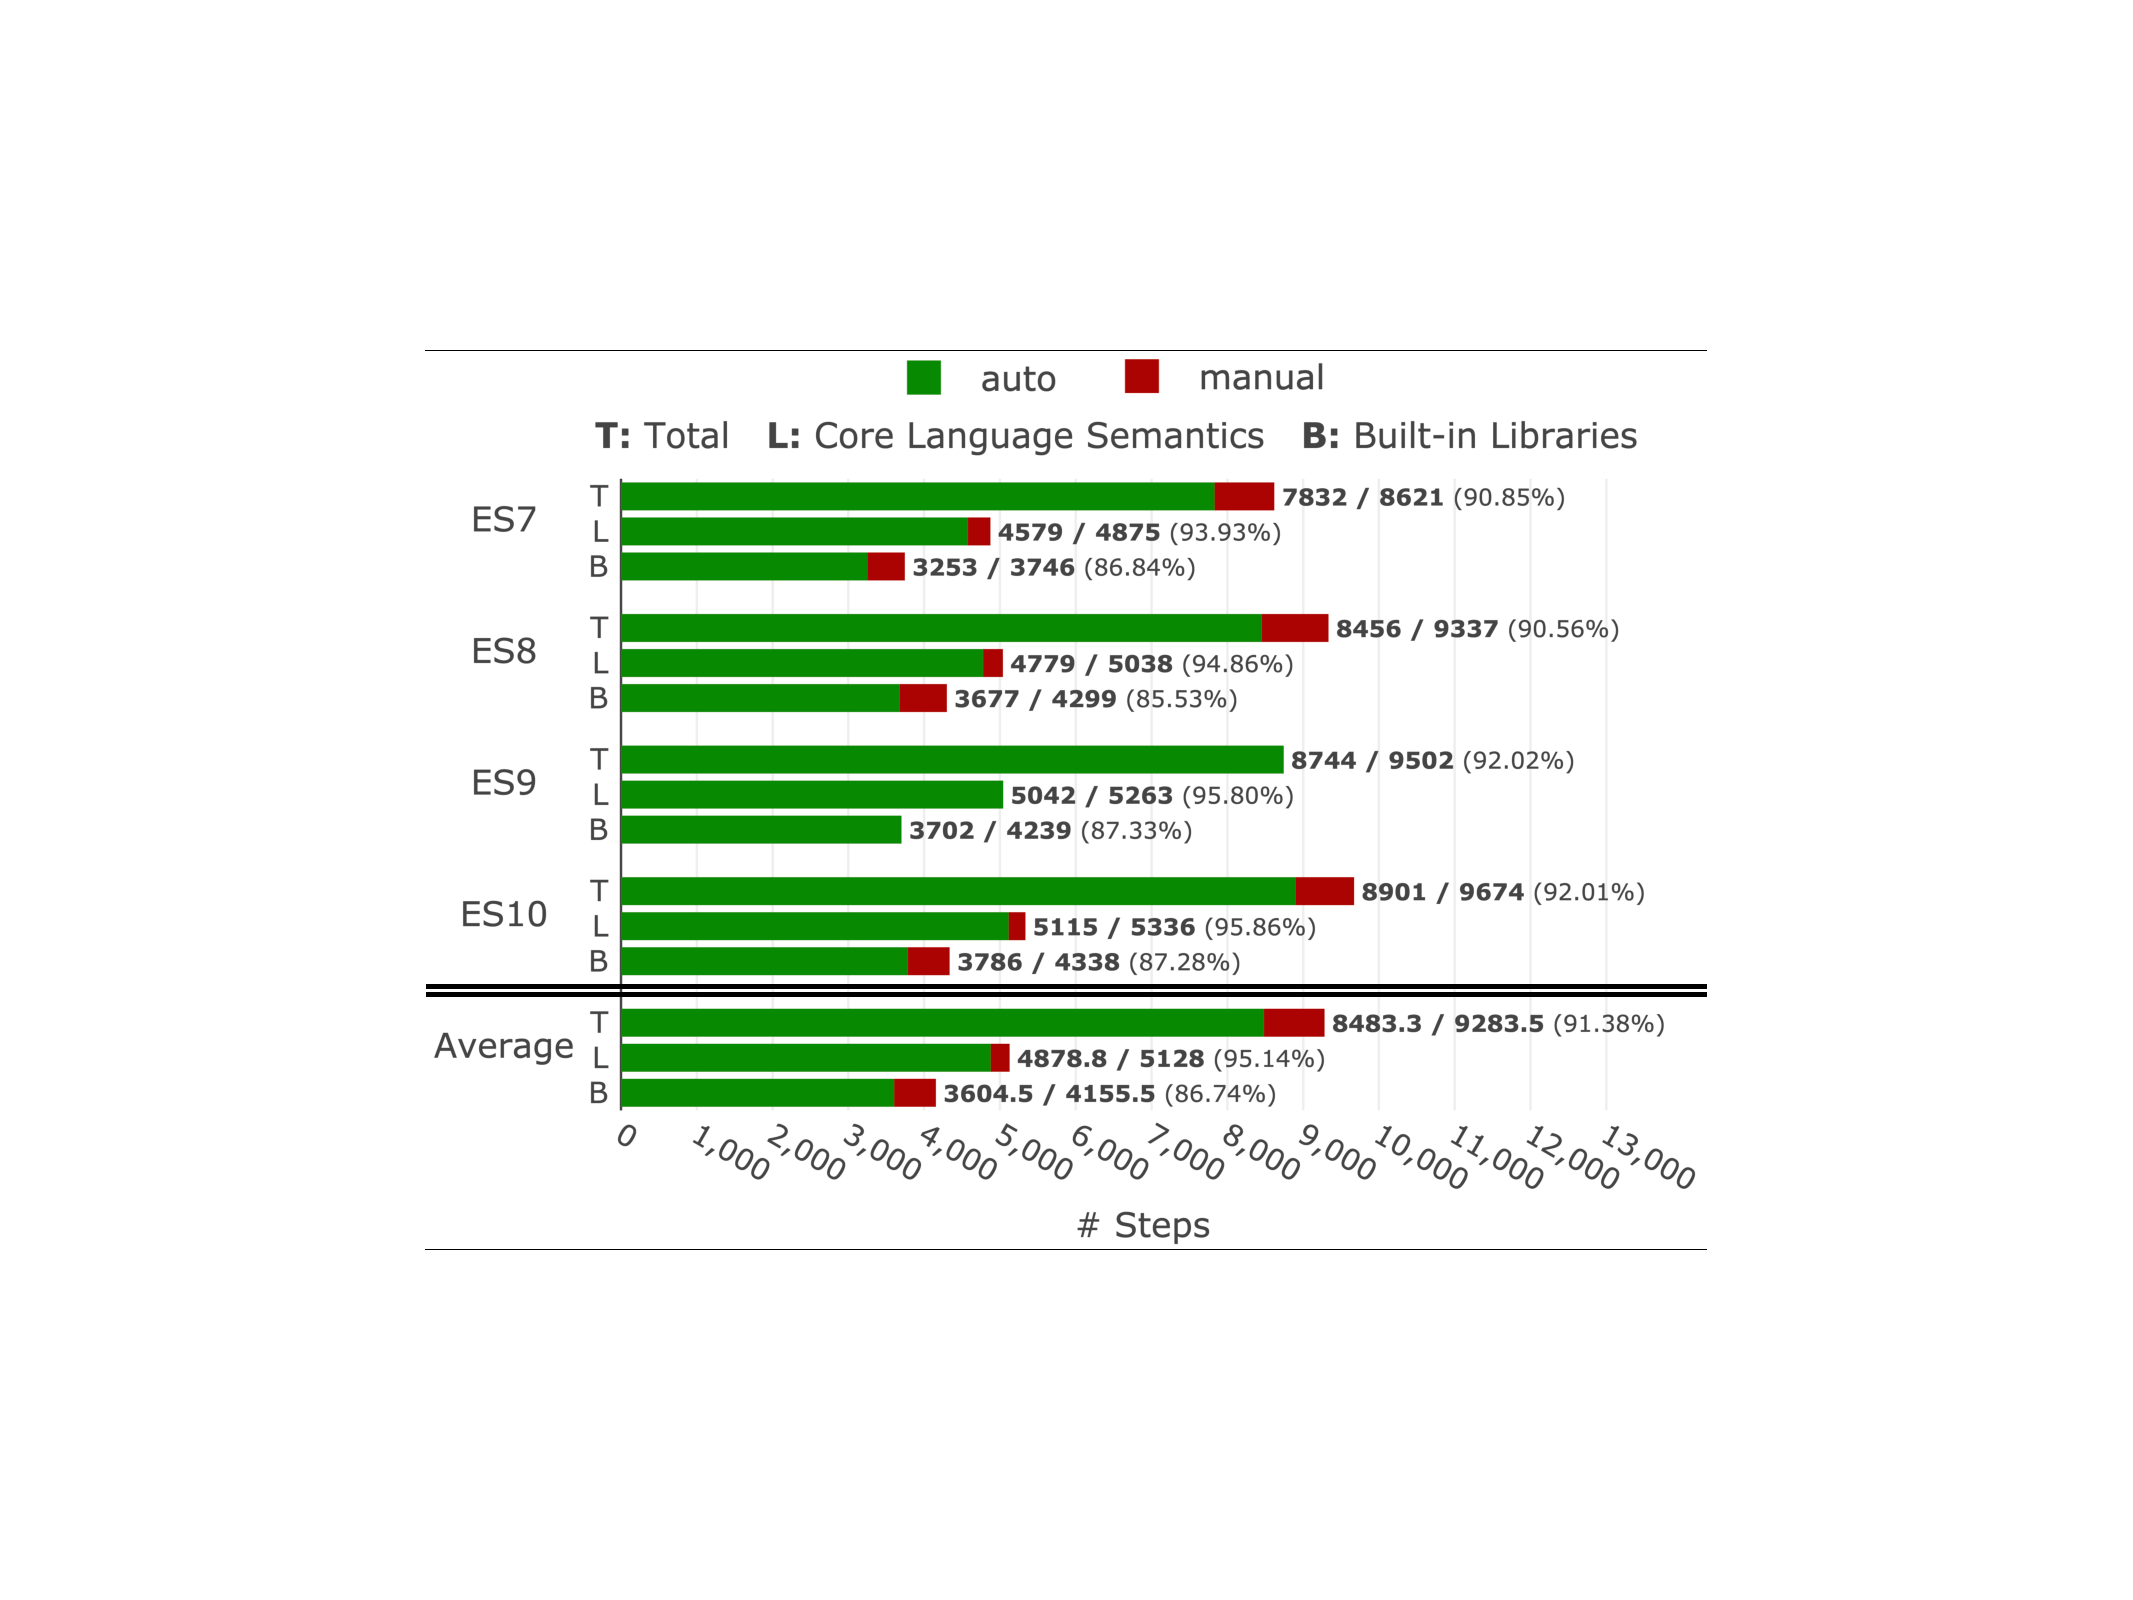
\includegraphics[width=\textwidth]{img/sem-all.pdf}
    \caption{Results for existing versions}
    \label{fig:semantics-all-version}
  \end{subfigure}
  \hfill
  \begin{subfigure}{0.48\textwidth}
    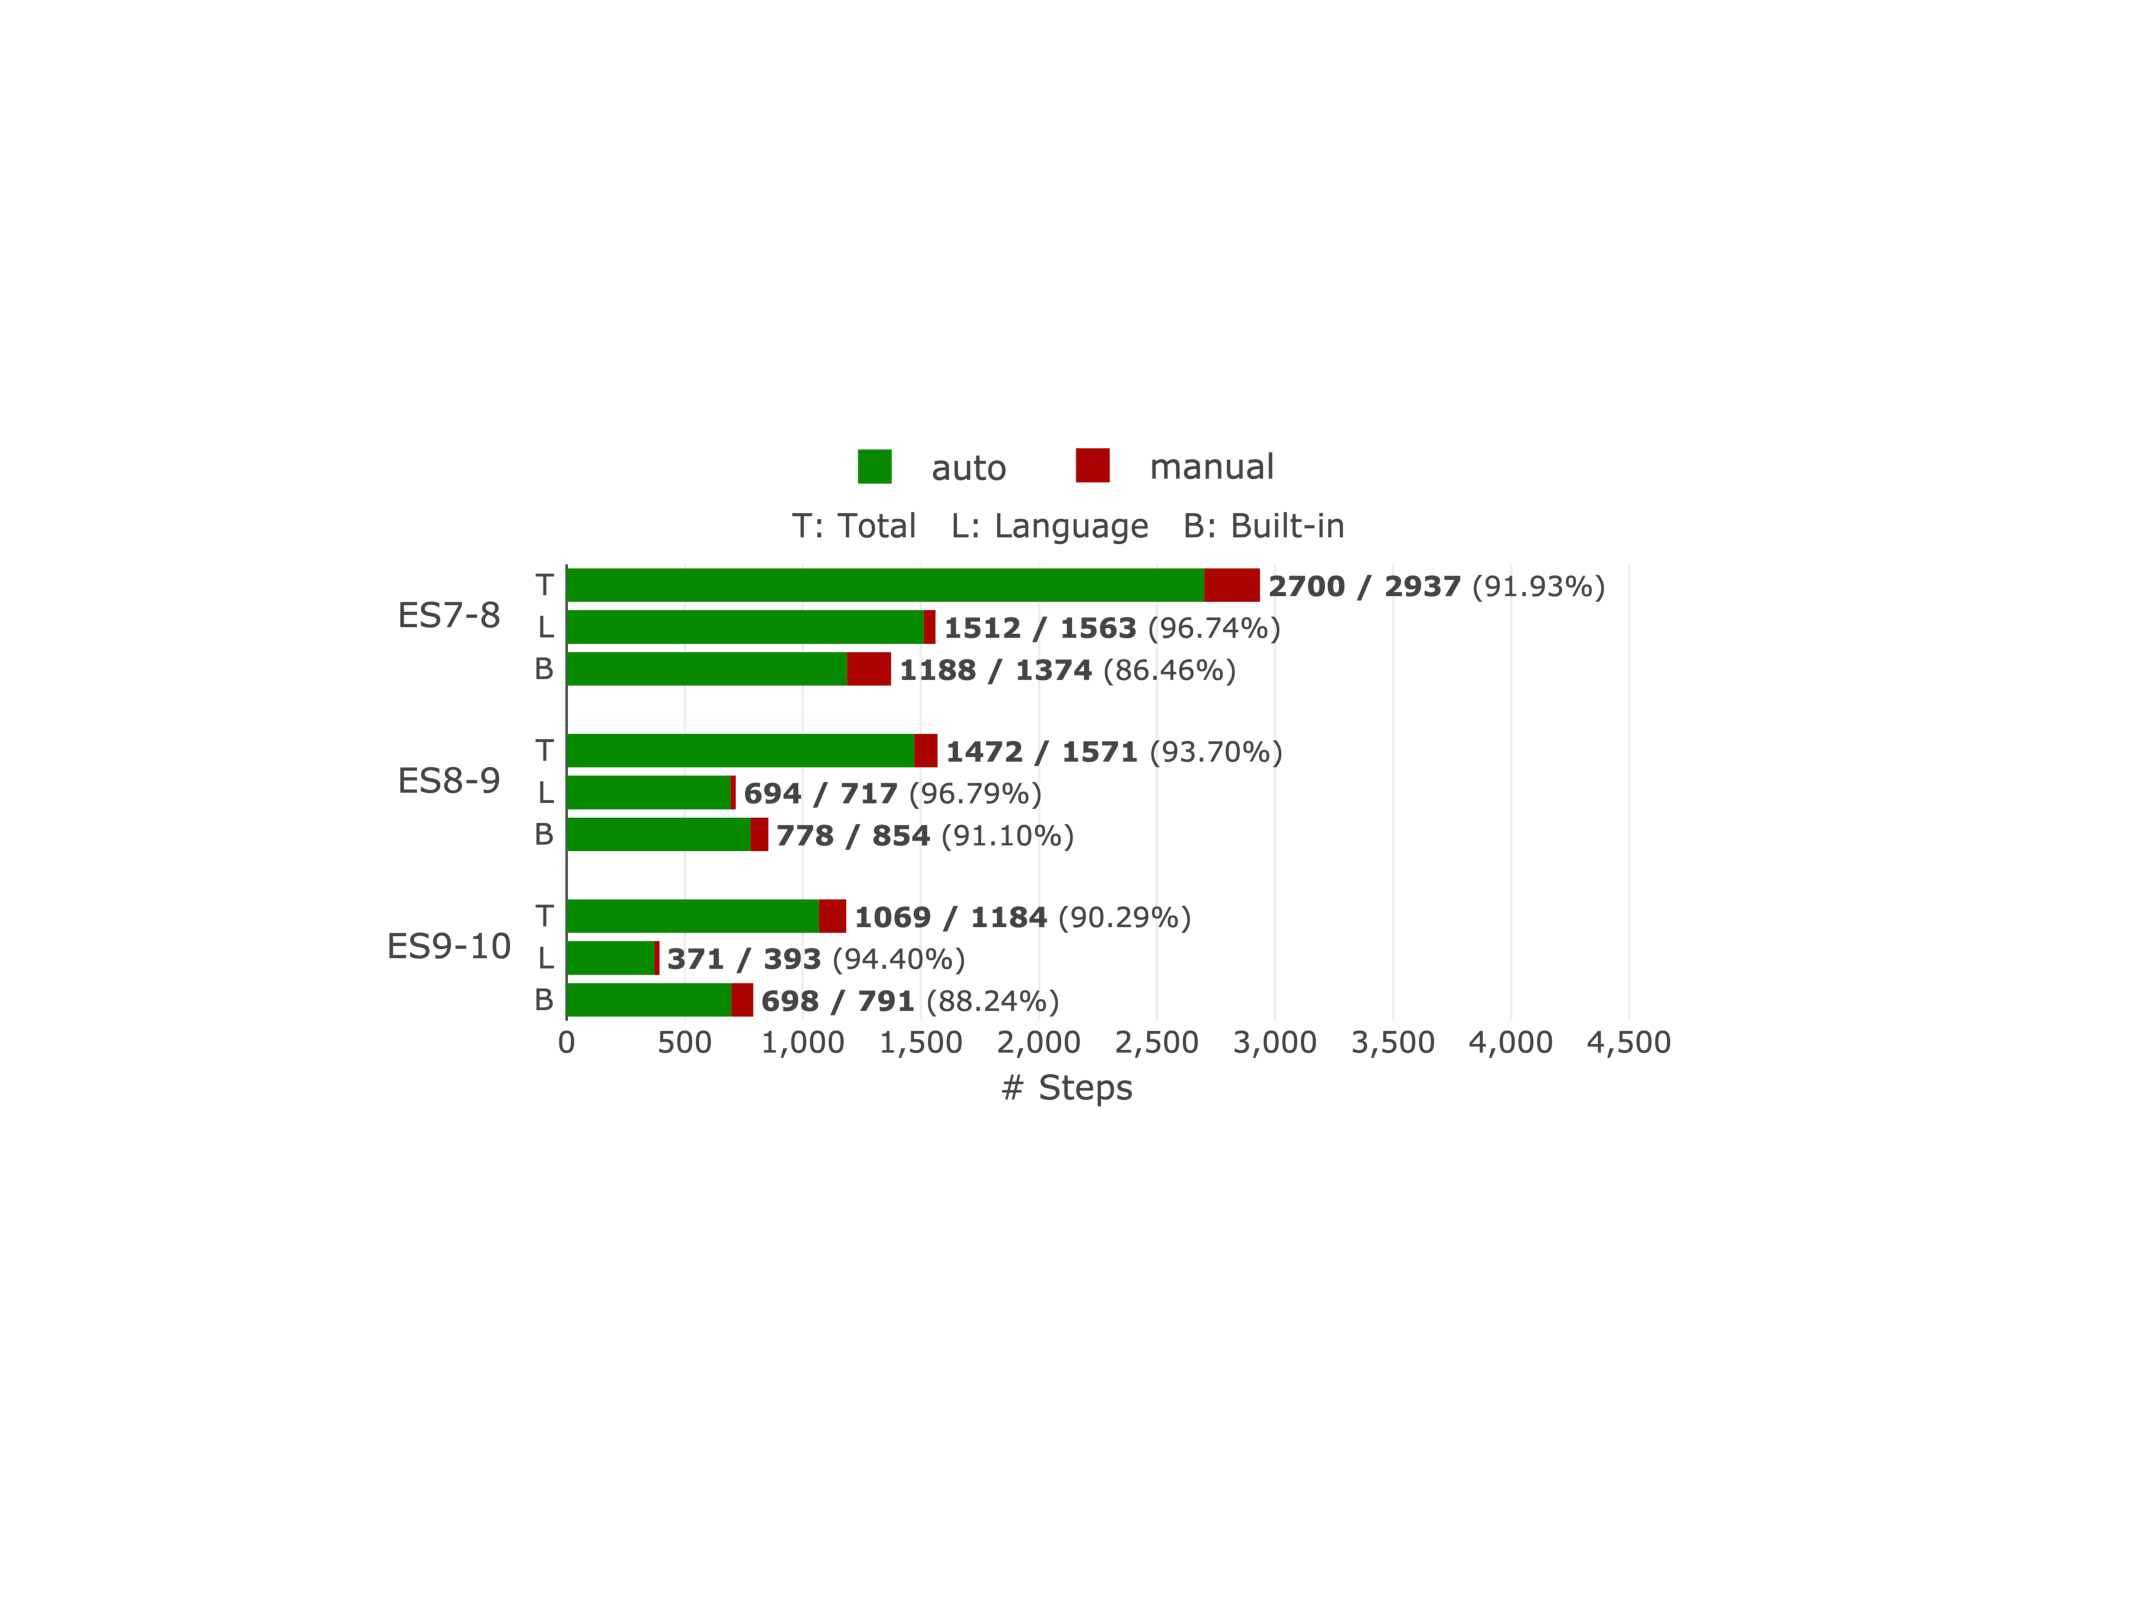
\includegraphics[width=\textwidth]{img/sem-diff.pdf}
    \caption{Results for differences between adjacent versions}
    \label{fig:semantics-all-version-diff}
  \end{subfigure}
  \caption{Number of abstract algorithm steps in specifications, from which
\( \tool \) generated the JavaScript semantics}
  \label{fig:all-version}
\vspace*{-1em}
\end{figure}

For semantics, Figure~\ref{fig:all-version} shows that \( \tool \) automatically
compile algorithm steps to the corresponding \( \ires \) instructions with
\inred{91.60\%} success rate on average for existing specifications, and
\inred{90.43\%} for updates.  ECMAScript abstract algorithms describe not only
core language semantics but also other helper functions of built-in libraries.
Built-in libraries written in more diverse styles in describing their own
specific functionalities.  Thus, built-in libraries have lower success rates
(\inred{86.98\%} for specifications and \inred{86.09\%} for updates) than core
language semantics (\inred{95.35\%} for specifications and \inred{95.25\%} for
updates).

This results show that \( \tool \) effectively reduces the efforts to
extract the syntax and semantics of JavaScript not only for developing
them from scratch, but also for updating existing ones.


\subsection{Check with Tests}\label{sec:check-with-tests}

To define the \textit{first IR-based formal semantics of modern JavaScript}, we
completed missing parts of the AST-IR translator for ES10.  Among \inred{9,674}
steps in ES10, \inred{8,901} steps are automatically compiled via
\textsf{Algorithm Compiler}.  Among the remaining \inred{773} steps, we manually
implemented all remaining language semantics (\inred{221} steps) and essential
parts of built-in libraries (\inred{XX} steps out of \inred{552}) in \inred{XX}
days.  Moreover, we manually implemented the \textsf{Global Setting} as described
in Section~\ref{sec:compiler-impl} for the core language features.  However, we
do not support several minor language features that do not affect the overall
JavaScript semantics critically: non-strict mode codes, modules, early errors
before actual executions, and inessential built-in objects.

Thanks to the executability of our extracted formal semantics, we checked the
semantics with Test262, the official conformance test suite provided by TC39.
We fixed version of Test262 as of February 28, 2019 because the ES10 was
branched out with the branch name es2019 in that day.  While it consists of
\inred{XX,XXX} tests, we filtered out \inred{XX,XXX} tests not applicable for
our formal semantics as shown in Table~\ref{table:test262}.  Test262 targets not
only the current official version of ECMAScript but several extensions and
in-progress features. We excluded \inred{X,XXX} tests for such cases to focus on
the semantics of ES10.  Among \inred{XX,XXX} ES10 tests, we also filtered out
\inred{X,XXX} tests using language features not supported by our semantics.

\begin{table*}[t]
  \centering
  \caption{Specification errors and wrong tests in Test262.}
  \label{table:spec-tests-errors}
  \vspace*{-0.5em}
  \small
  \begin{tabular}{|c|c|l|c|c|c|c|c|}
    \hline
    \multicolumn{1}{|c|}{\bf Name} &
    \multicolumn{1}{c|}{\bf Feature} &
    \multicolumn{1}{c|}{\bf Description} &
    \multicolumn{1}{c|}{\bf Known} &
    \multicolumn{1}{c|}{\bf Created} &
    \multicolumn{1}{c|}{\bf Resolved} &
    \multicolumn{1}{c|}{\bf Existed} &
    \multicolumn{1}{c|}{\bf \# Failed Tests} \\\hline

    es10-1 &
    Await &
    \makecell[l]{Passing wrong type of \\ the second argument for {\bf PromiseResolve}.} &
    \textsf{O} &
    2019-02-27 &
    2019-04-13 &
    45 days &
    \inred{XX} \\\hline

    es10-2 &
    IterationKind &
    \makecell[l]{Missing \code{async-iterate} case \\ in the assertion of {\bf
    ForIn/OfHeadEvaluation}.} &
    \textsf{X} &
    2018-02-16 &
    2020-03-25 &
    768 days &
    \inred{XX} \\\hline

    es10-3 &
    Completion &
    \makecell[l]{Not handling abrupt completion \\ in {\bf Evaluation} of {\it
    EqualityExpression}.} &
    \textsf{O} &
    2016-06-01 &
    2019-05-02 &
    1065 days &
    \inred{XX} \\\hline

    es10-4 &
    Function &
    \makecell[l]{No semantics of {\bf IsFunctionDefinition} \\ for
    \code{function(...)\{...\}}.} &
    \textsf{O} &
    2015-10-30 &
    2020-01-18 &
    1541 days &
    \inred{XX} \\\hline

    es10-5 &
    ForOf &
    \makecell[l]{Two semantics of {\bf VarScopedDeclarations} \\ for \code{for
    await(var x of e)\{...\}}.} &
    \textsf{O} &
    2018-02-16 &
    2019-10-11 &
    602 days &
    \inred{XX} \\\hline

    es10-6 &
    Argument &
    \makecell[l]{No semantics of {\bf ExpectedArgumentCount} \\ for the base case
    of {\it FormalParameters}.} &
    \textsf{O} &
    2016-11-02 &
    2020-02-20 &
    1205 days &
    \inred{XX} \\\hline

    es10-7 &
    String &
    \makecell[l]{Wrong use of \code{=} operator in {\bf
    StringGetOwnProperty}.} &
    \textsf{X} &
    2015-06-01 &
    \inred{2019-00-00} &
    \inred{XX} days &
    \inred{XX} \\\hline

    test-1 &
    Global &
    \makecell[l]{Testing implementation-dependent [[Prototype]] \\ of the global
    object.} &
    \textsf{X} &
    \inred{2019-00-00} &
    \inred{2019-00-00} &
    \inred{XX} days &
    10 \\\hline

    bigint-1 &
    UpdateExpression &
    \makecell[l]{Using wrong variable \code{oldvalue} instead of \\
    \code{oldValue} in {\bf Evaluation} of {\it UpdateExpression}.} &
    \textsf{X} &
    2019-09-27 &
    2020-04-23 &
    209 days &
    \inred{XX} \\\hline

    bigint-2 &
    NumberOp &
    \makecell[l]{Using {\bf ToInt32} instead of {\bf ToUint32} \\ in {\bf
    Number::unsignedRightShift}.} &
    \textsf{X} &
    2019-09-27 &
    2020-04-23 &
    209 days &
    \inred{XX} \\\hline

    bigint-3 &
    NumberOp &
    \makecell[l]{Using {\bf ToUint32} instead of {\bf ToInt32} \\ in {\bf
    NumberBitwiseOp}.} &
    \textsf{X} &
    2019-09-27 &
    2020-04-23 &
    209 days &
    \inred{XX} \\\hline

    bigint-4 &
    Number &
    \makecell[l]{Not handling BigInt values in {\bf Number} constructor.} &
    \textsf{O} &
    2019-09-27 &
    2019-11-19 &
    53 days &
    \inred{XX} \\\hline

  \end{tabular}
\end{table*}

\begin{table}[t]
  \centering
  \caption{Excluded tests in Test262}
  \label{table:test262}
  \vspace*{-0.5em}
  \small
  \begin{tabular}{lr}\toprule
    \belowrulesepcolor{gainsboro}
    \rowcolor{gainsboro} \textbf{All Test262 Tests} & \inred{\textbf{XX,XXX}}\\
    \aboverulesepcolor{gainsboro}\midrule
    Annexes & \inred{XXX}\\\hdashline
    Internationalization & \inred{XXX}\\\hdashline
    In-progress features & \inred{X,XXX}\\\midrule
    \belowrulesepcolor{gainsboro}
    \rowcolor{gainsboro} \textbf{ES10 Tests} & \inred{\textbf{XX,XXX}}\\
    \aboverulesepcolor{gainsboro}\midrule
    Non-strict modes & \inred{X,XXX}\\\hdashline
    Modules & \inred{X,XXX} \\\hdashline
    Early errors & \inred{X,XXX} \\\hdashline
    Inessential built-in objects & \inred{X,XXX} \\\midrule
    \belowrulesepcolor{gainsboro}
    \rowcolor{gainsboro} \textbf{Applicable Tests} & \inred{\textbf{XX,XXX}}\\
    \aboverulesepcolor{gainsboro}\midrule
    Passed tests & \inred{XX,XXX} \\\hdashline
    Failed tests & \inred{XXX} \\\bottomrule
  \end{tabular}
  \vspace*{-2em}
\end{table}

For \inred{XX,XXX} applicable tests, the synthesized JavaScript parser
successfully parses all tests but \inred{XXX} tests are failed to be executed
because of the different semantics between ECMAScript and official tests.  Based
on the failed tests, we found 7 specification errors in ES10 and 10 wrong tests
in Test262 as described in Table~\ref{table:spec-tests-errors}.  For example,
the specification error es10-1 is related to the JavaScript Await.  The {\bf
PromiseResolve (C, x)} algorithm creates a new Promise object using a given
constructor {\bf C} and resolved with a given value {\bf x}.  However, a
specification update added three invocations of {\bf PromiseResolve} with a list
of values for {\bf x} in February 27, 2019.  This error exists in 45 days until
April 13, 2019 and fails \inred{XX} tests for ES10 in Test262.  For other cases,
es10-2 arises because of the wrong assertion. es10-3 and es10-7 arise because
contributors misunderstood the meaning of abrupt completion and \code{=}
operator for numbers, respectively.  es10-4, es10-5, and es10-6 are
specification errors that miss or define twice specific corner cases of
semantic.  For example, es10-4 is an error that does not define the {\bf
IsFunctionDefinition} algorithm for unnamed functions such as
\code{function(){}}.  For these seven specification errors, they existed in ES10
in \inred{XXX} days on average.  Besides, two errors es10-2 and es10-7 are even
not known before we reported to TC39.

For tests in Test262, we found 10 wrong tests categorized in test-1 and they are
related to the JavaScript global object. The [[Prototype]] internal property of
the global object is fully implementation dependent thus the official tests
should not check its attributes.  However, 10 tests assumes that [[Prototype]]
of the global object is a prototype chain starts with \code{Object.prototype}.
They violate the implementation dependent semantics of ES10.  Moreover, they
existed in Test262 in \inred{XXX} days.

After resolving above specification errors in ES10, we extracted formal
semantics from the revised specification again. The revised formal semantics of
ES10 passed all \inred{XX,XXX} applicable tests in Test262.  We believe that our
tool can assist to check and find bugs in ECMAScript by generating executable
formal semantics and executing it with tests in Test262.


\subsection{Forward Compatibility}

We show the forward compatibility of \( \tool \) by applying it to the proposals
that are ready for inclusion in the next ECMAScript (ES11, 2020). Because
ECMAScript administered as an open-source project, various proposals for new
language features are available with their own specification changes and tests.
A separate repository~\cite{proposals} maintains such proposals with six
different stages: Stage 0 to Stage 3, Finished, and Inactive.  Each proposal
starts with Stage 0, and the TC39 committee regularly examines Stage 3 proposals
to decide their next stages.  If a proposal is confirmed, the committee changes
its stage to Finished and integrates it into the next version of ECMAScript.
Otherwise, the committee changes its stage to Inactive.  Among them, we applied
\( \tool \) to all Finished proposals decided to be included in ES11.

\begin{table}[t]
  \centering
  \caption{Evaluation result of \( \tool \) for Finished stage proposals that
  will be included in ES11.}
  \label{table:spec-prop-result}
  \vspace*{-0.5em}
  \small
  \begin{tabular}{c?r|r?r?r}
    \hline
    \multicolumn{1}{c?}{\multirow{2}{*}{\bf Name}} &
    \multicolumn{2}{c?}{\bf \( \Delta \) \# Prod.} &
    \multicolumn{1}{c?}{\multirow{2}{*}{\bf \( \Delta \) \# Steps}} &
    \multicolumn{1}{c}{\multirow{2}{*}{\bf \# Tests}} \\\cline{2-3}

    &
    \multicolumn{1}{c|}{\bf Lex.} &
    \multicolumn{1}{c?}{\bf Syn.} &
    &\\\hline\hline

    \code{matchAll} of \code{String} &
    \inred{X} &
    \inred{X} &
    9/9 &
    5/5\\\hline

    \code{import()} &
    \inred{X} &
    \inred{X} &
    \inred{X/X} &
    \inred{X/X}\\\hline

    \code{BigInt} &
    \inred{X} &
    \inred{X} &
    258/323 &
    \inred{207}/207\\\hline

    \code{Promise.allSettled} &
    \inred{X} &
    \inred{X} &
    79/85 &
    50/50\\\hline

    \code{globalThis} &
    \inred{X} &
    \inred{X} &
    1/1 &
    1/1\\\hline

    \code{for-in} mechanics &
    \inred{X} &
    \inred{X} &
    \inred{X/X} &
    \inred{X/X}\\\hline

    Optional Chaining &
    \inred{X} &
    \inred{X} &
    72/74 &
    19/19\\\hline

    Nullish Coalescing Op. &
    \inred{X} &
    \inred{X} &
    10/10 &
    21/21\\\hline

    \code{import.meta} &
    \inred{X} &
    \inred{X} &
    \inred{X/X} &
    \inred{X/X}\\\hline

    {\bf Total} &
    \inred{X} &
    \inred{X} &
    \inred{X/X} &
    \inred{X/X}\\\hline
  \end{tabular}
\end{table}

Table~\ref{table:spec-prop-result} shows the result of applying \( \tool \) to 9
Finished proposals for ES11.  For all proposals, \inred{XX} lexical and
\inred{XX} syntactic productions are modified and \( \tool \) successfully
updated the changes to the synthesized JavaScript parser.  The updated parser
parses all applicable tests for all proposals.  For abstract algorithms,
\inred{XXX} steps out of \inred{XXX} steps are automatically converted to the
corresponding \( \ires \) instructions by the algorithm compiler without
changing of the compile rules.  Thus, our tool has \inred{XX.XX\%} success rate
on average for future proposals.  Similar with
Section~\ref{sec:check-with-tests}, we manually implemented missing part of the
AST-IR translator for each Finished proposal and checked each extracted
semantics with official tests.  Each of them passed all applicable tests except
the semantics for \code{BigInt} proposal.  It fails \inred{XX} tests out of 207
applicable tests.

Based on the failed tests, we found three undiscovered specification errors
(bigint-1, bigint-2, and bigint-3), and one reported error (bigint-4) in the
BigInt proposal as described in Table~\ref{table:spec-tests-errors}.  All of
them were confirmed by TC39 and will be fixed in the next release.  The BigInt
proposal added a new type of primitives BigInt and unified the type with
original Number type to Numeric types.  Thus, it not only added new
algorithms for BigInt but also modified all existing algorithms related to
number values.  The error bigint-1 is just a simple misuse of the variable
\code{oldValue} in {\bf Evaluation} of {\it UpdateExpression}. bigint-2 and
bigint-3 break the backward compatibility because of the incorrectly mixed uses
of {\bf ToInt32} and {\bf ToUint32} algorithms in unsigned right shift operators
and bitwise operators, respectively. The last one bigint-4 arises because the
Number constructor does not consider BigInt primitives.  On average, ECMAScript
included these four specification errors in \inred{XXX} days.

After fixing all specification errors, we extracted the semantics for the BigInt
proposal again.  The updated semantics passed all 207 applicable tests.  Thus,
\( \tool \) also correctly extract IR-based semantics from future proposals.

\section{Related Work}\label{sec:related}

Type analysis of JavaScript specifications has three related topics:
JavaScript tools, mechanized specification extraction, and specification-based testing.

\paragraph{JavaScript Tools}
ECMAScript is the standard language specification for JavaScript maintained by
TC39.  In late 2014, the committee announced
its plan to release ECMAScript annually and adopt the open development process
to quickly adapt to evolving development environments.  Various JavaScript engines such
as Google V8~\cite{v8}, GraalJS~\cite{graaljs}, QuickJS~\cite{qjs}, and Moddable
XS~\cite{moddable} should conform to the syntax and semantics described in
annually updated ECMAScript.  Beyond JavaScript engines, diverse
research projects use JavaScript specifications.  The main research direction
has been static analyzers such as JSAI~\cite{jsai}, SAFE~\cite{safe},
TAJS~\cite{tajs}, and WALA~\cite{wala} based on the abstract interpretation
framework~\cite{ai1977, ai1992} with their own analysis techniques.
They defined abstract semantics of the JavaScript semantics described in ECMAScript to statically
analyze JavaScript programs in a finite time.
Chargu{\'e}raud et al.~\cite{jsexplain} presented JSExplain, a debugger for JavaScript, by
implementing a reference interpreter in OCaml following the algorithm steps in ECMAScript closely.
For a given JavaScript program, the debugger interactively produces execution traces
investigated in a browser, with an interface that displays the
JavaScript code and the interpreter's state.
Fragoso Santos et al.~\cite{javert} introduced JaVerT, a JavaScript verification toolchain, based
on the separation logic with an intermediate goto language JSIL.
JaVerT 2.0~\cite{javert2} extends it to support compositional symbolic execution
for JavaScript based on bi-abduction.  However, because all of them manually handle
ECMAScript with their own intermediate representations, most of them still 
target ES5.1 released in 2011 instead of the latest one.

\paragraph{Mechanized Specification Extraction}
Researchers in various application domains have extracted mechanized specifications from
specifications written in natural languages to handle the contents in the specifications automatically.
For system architectures, researchers utilized Natural
Language Processing (NLP) and Machine Learning techniques to extract formal semantics
of small-sized low-level assembly languages for x86~\cite{x86} and ARM~\cite{arm}.
For Java API functions, Zhai et al.~\cite{javadoc} presented a
technique to automatically extract models from their documentation using NLP techniques.
For the JavaScript programming language, Park et al.~\cite{jiset}
presented $\jiset$, a tool that extracts a mechanized specification from ECMAScript.
While all the previous JavaScript formal semantics~\cite{lambdajs, jscert,
kjs} were manually defined, $\jiset$ automatically extracts formal semantics directly from ECMAScript.
We utilized $\jiset$ to analyze 864 ECMAScript versions via $\tool$.

\paragraph{Specification-based Testing}
Recently, researchers have utilized specifications to test their implementations.
For network protocols, Kim et al.~\cite{basespec} proposed a novel approach named
\textsc{BaseSpec}, which extracts message structures from tables in cellular
specifications for L3 protocols to perform comparative analysis of baseband software.
Schumi and Sun~\cite{spectest} presented SpecTest, which utilized an
executable language semantics to perform fuzzing for Java and Solidity compilers.
For JavaScript, Ye et al.~\cite{comfort} presented \textsc{Comfort}, a
compiler fuzzing framework to detect JavaScript engine bugs using ECMAScript
with deep learning-based language models.
Park et al.~\cite{jest} extended $\jiset$ to $\jest$, which performs $N$+1-version differential testing
with $N$ different JavaScript engines and a reference interpreter extracted from ECMAScript.
$\jest$ detects not only engine bugs but also specification bugs in
ECMAScript using the cross-referencing oracle.  However, it requires multiple JavaScript engines and
takes dozens of hours to test a version of ECMAScript.
Instead, $\tool$ can detect specification bugs without JavaScript engines in two minutes.
Because $\tool$ uses abstract semantics while $\jest$ uses concrete semantics,
$\tool$ can quickly analyze more scope of semantics than $\jest$.

\section{Conclusion}\label{sec:conclusion}
Since an incorrect description in ECMAScript can lead to the wrong JavaScript
engine implementations, checking the correctness of ECMAScript is essential.
Since ECMAScript is annually released and developed in open process, it becomes
more labor-intensive and error-prone.  To alleviate the problem, we propose
$\tool$, a JavaScript Specification Type Analyzer using Refinement.  It is the
first tool that performs \textit{type analysis} on JavaScript specifications and
detects specification bugs using a \textit{bug detector}.  Moreover, to increase
precision of type analysis, we present \textit{condition-based refinement} for
type analysis, which prunes out infeasible abstract states using conditions of
assertions and branches.  We evaluated $\tool$ with all 864 versions in the
official ECMAScript repository for the recent three years from 2018 to 2021.
Our tool took \inred{137.3} seconds on average to perform type analysis for each
version, and detected \inred{161} type-related specification bugs with
\inred{56.5}\% precision; \inred{91} out of \inred{161} bugs are true bugs.
Among them, \inred{14} bugs are newly detected by $\tool$, and the committee
confirmed all of them.


\bibliographystyle{ACM-Reference-Format}
\bibliography{ref}

\end{document}
